\documentclass[																					%IRAS Vorlage
  a4paper,
  oneside,
  nexus,
  11pt,																									% <10pt, 9pt>
																												%style=screen,
																												%sender=bottom,
  blue,																									% <orange, green, violet>
																												%rgb, <cmyk>
																												%mono,
																												%extramargin,
																												%marginleft, <marginright>
  ]{tubsreprt}

\usepackage[utf8x]{inputenc}
\usepackage[ngerman]{babel}
\usepackage[square]{natbib}
\usepackage{graphicx}
\usepackage{amsmath}                   									 % Packages für Formeln
\usepackage{amsthm}																			 % -||-
\usepackage{amsfonts}																		 % -||-
\usepackage{amssymb}																		 % -||-
\usepackage{lscape} 																			% Querformatiges Beschreiben einzelner Abschnitte %mit \begin{landscape} Text \end{landscape}
\usepackage{siunitx}																		 %si-einheiten
\sisetup{locale = DE}																			%Deutsche Dezimalzahlkonvention
\DeclareSIUnit\unit{U}																	%CubeSat Unit[U] als Einheit definiert
																												
																												

\usepackage{tikz} 																			 % TikZ - ein geniales Zeichentool vor allem für Skizzen oder Schemata, Programmabläufe, etc.
\usepackage{bibgerm}																		%bibliography deutsch
																										 
\usepackage{pgf}																				 % Für Tikz
\usepackage{pgfplots} 																	 % Plots mit TikZ
\usetikzlibrary{shapes, backgrounds, arrows, positioning, trees, shadows}% Bibliotheken für Tikz
\usepackage{pgfgantt}																		 % Zum Erstellen eines Gantt-Charts

\graphicspath{{./graphics/}}														 %greift auf den Unterordner "graphics" zu
\usepackage{pdfpages}																		 %ermöglicht das Einbinden von PDF-Datein
\usepackage{float}

%===============================================================
%
%	Hyperlinks im Dokument
%
%---------------------------------------

\usepackage[
	pdftex,
  hidelinks,%
  linktocpage, breaklinks
]{hyperref}																							% Package für Lesezeichen und Verlinkungen

%===============================================================
%
%	Glossary
%
%---------------------------------------
\usepackage[nonumberlist,acronym,section]{glossaries}

 
																												%nonumberlist: no page numbering
																												%acronym: abbreviations list
																												%toc: entry in table of contents
																												%section: in toc placed at section level
																												%nopostdot: no dots after description
				
\newglossary[slg1]{symbolslist}{syi}{syg}{List of Symbols}																			% symbols
\newglossary[alg]{acronymlist}{acr}{acn}{List of Abbreviations}																	% abbreviations	

\makeglossaries

\AtEndDocument{\glsaddall}																%füge alle Symbole dem Verzeichnis zu

%-----------------------------------------------------------------


																													%Makros für eine erleichterte Eingabe wiederkehrender Befehle:
\newcommand{\abb}[1]{Abbildung~\ref{#1}}
\newcommand{\tab}[1]{Tabelle~\ref{#1}}
\newcommand{\glg}[1]{Gleichung~\ref{#1}}
\newcommand{\kap}[1]{Kapitel~\ref{#1}}
\newcommand{\abschn}[1]{Abschnitt~\ref{#1}}
\newcommand{\anh}[1]{Anhang~\ref{#1}}

\newcommand{\ul}{\underline}
\newcommand{\ol}{\overline}
\newcommand{\tb}{\textbf}
\newcommand{\ts}{\textsl}

\newcommand{\kalman}{\textsc{Kalman}-Filter }

%===============================================================
%
% Farben
%
%-------------------------------

\definecolor{ilr-blue}{RGB}{44,79,162}
\definecolor{light-blue}{RGB}{220,220,255}
\definecolor{gray90}{gray}{0.9}
\definecolor{gray80}{gray}{0.8}
\definecolor{gray60}{gray}{0.6}
\definecolor{gray50}{gray}{0.5}
\definecolor{gray40}{gray}{0.4}
\definecolor{gray20}{gray}{0.2}

%===============================================================
%
% Titelseiten
%
%-------------------------------

\title{\LARGE Projektarbeit SS 2019 \newline Analyse einer CubeSat-basierten ADR-Mission}
\subtitle{Institut f\"ur Raumfahrtsysteme}
\author{\small Florian Czorny, Frederik Sch\"afer, Marc Strempel, Oussama Mouhaya, Valentina Dietrich}

%---------------------------------------------------------------
% Titelbilder + IRAS Logo (Deckblatt)
%---------------------------------------------------------------

\logo{
\includegraphics{iras_logo.jpg}} 
\titlepicture{doctor_pop2009.jpg}

%===============================================================
% Hurenkind bzw. ein Schusterjunge 
%---------------------------------------------------------------
\clubpenalty         = 10000
\widowpenalty        = 10000
\displaywidowpenalty = 10000
%===============================================================
% Hauptfunktion
%---------------------------------------------------------------

\begin{document}																												%Erstellung des Schreibdokumentes 

  \maketitle[image] 																										%[<plain/image/imagetext>,<logo=left/right>]

 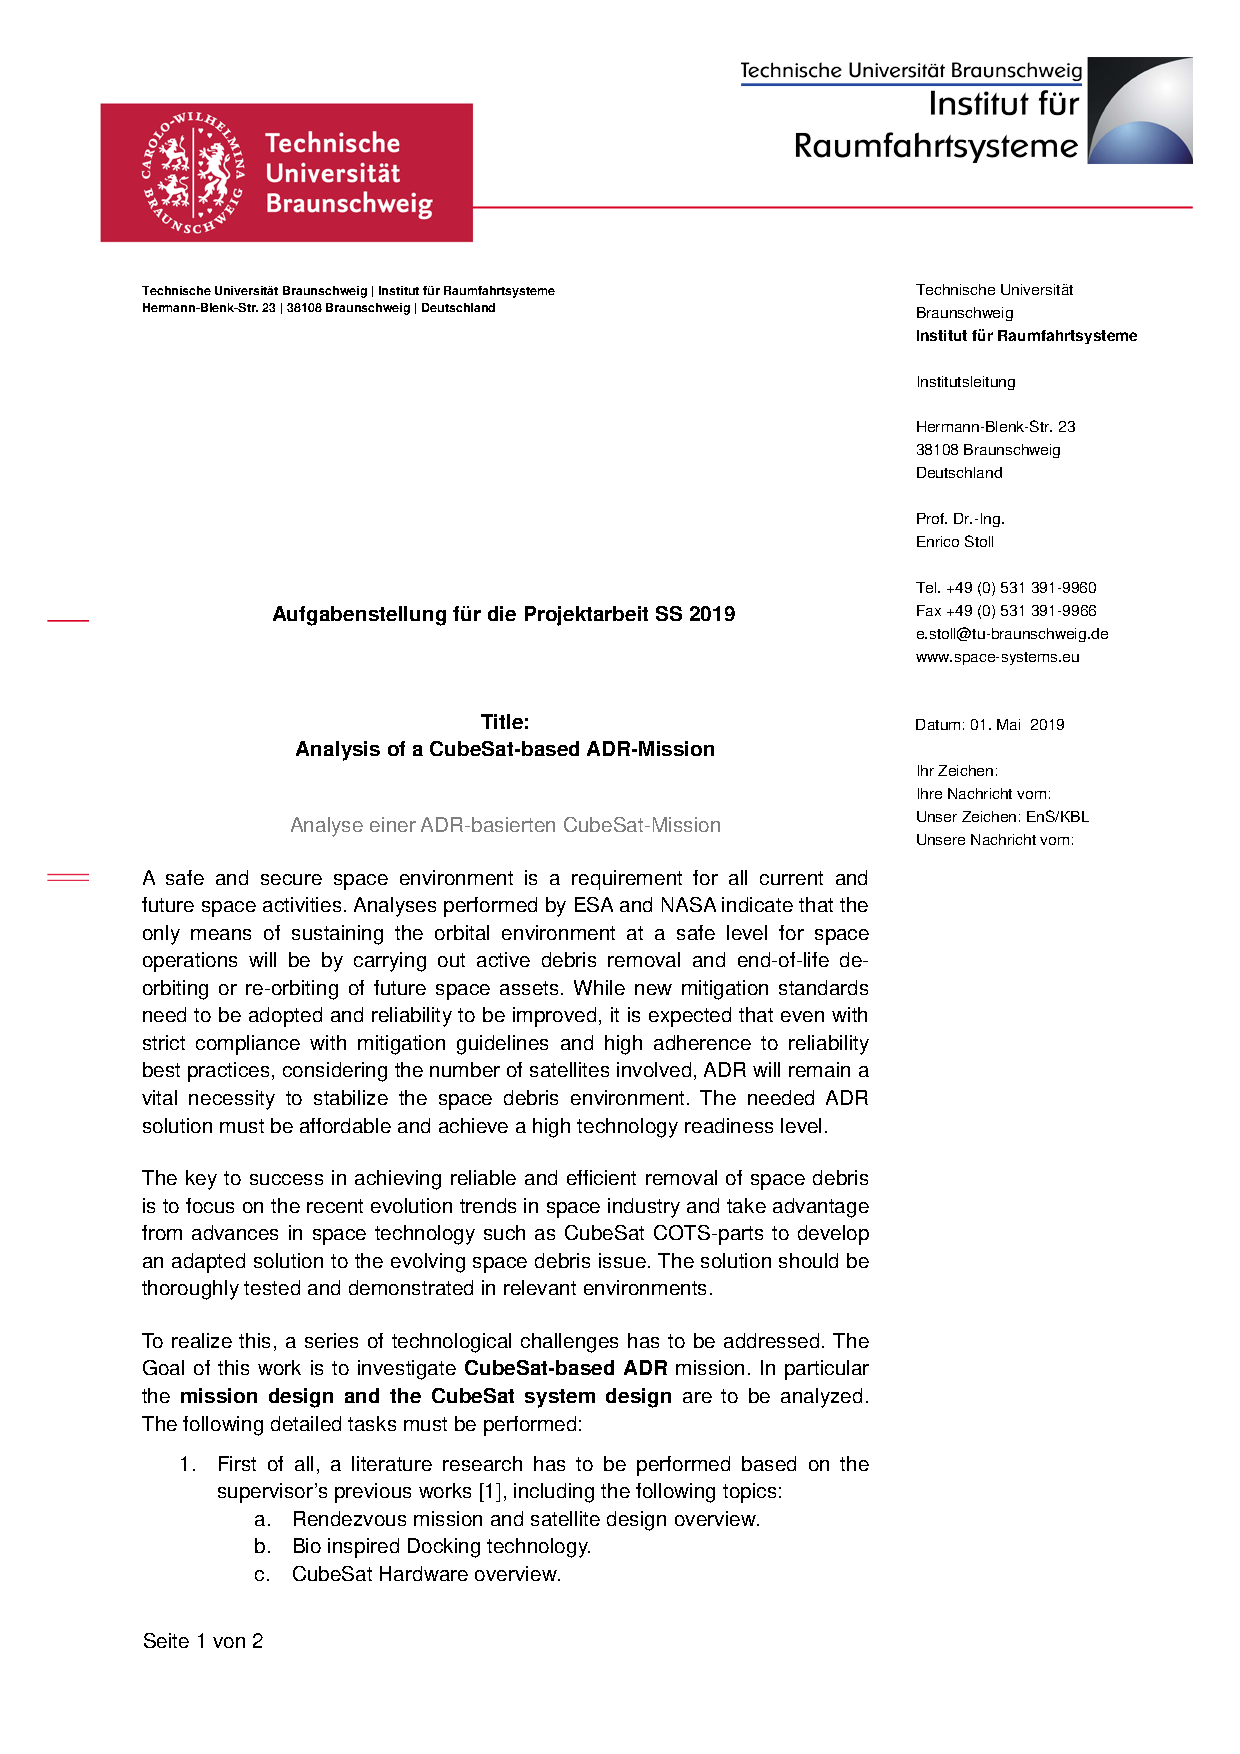
\includepdf[pages=-]{./header_first/Aufgabenstellung_PA_SS19.pdf}			%PDF-Datei wird hinzugefügt 
 \chapter*{Eidesstattliche Erkl\"arung}

Wir erklären hiermit an Eides Statt, dass wie die nachfolgende Arbeit selbständig und nur unter Zuhilfenahme der angegebenen Literatur angefertigt haben.


\vspace{2cm}
\tikz\draw (0,0) -- (7,0);

Datum, Unterschrift Florian Czorny
  
\vspace{2cm}
\tikz\draw (0,0) -- (7,0);

Datum, Unterschrift Frederik Schäfer
  
\vspace{2cm}
\tikz\draw (0,0) -- (7,0);

Datum, Unterschrift Marc Strempel

\vspace{2cm}
\tikz\draw (0,0) -- (7,0);

Datum, Unterschrift Oussama Mouhaya
 
\vspace{2cm}
\tikz\draw (0,0) -- (7,0);

Datum, Unterschrift Valentina Dietrich

 \tableofcontents																												%Erstellung eines Inhaltsverzeichnisses
  \newpage
	%\newglossarystyle{rhg-altlong4col}{\glossarystyle{altlong4col}
		\glossarystyle{altlong4col}
			\setlength{\glsdescwidth}{0.7\textwidth}
	
	%----------------------------------------------
%
% Symbolverzeichnis
%
%-----------------------------------------------


% LATIN (use prefix 'x' in sort)
%-----------------------

\newglossaryentry{symb:c} {name=\ensuremath{c},    description={Lichtgeschwindigkeit im Vakuum, \ensuremath{c=299.792.458\; \frac{m}{s}}}, 
symbol=\ensuremath{\frac{m}{s}},       sort=xc,type=symbolslist}
\newglossaryentry{symb:g} {name=\ensuremath{g},    description={Erdbeschleunigung}, symbol=\ensuremath{\frac{m}{s^{2}}},       sort=xg,type=symbolslist}
\newglossaryentry{symb:m} {name=\ensuremath{m},    description={Masse},             symbol=\ensuremath{kg},                    sort=xm,type=symbolslist}
\newglossaryentry{symb:E} {name=\ensuremath{E},    description={Energie},           symbol=\ensuremath{J},                     sort=xE,type=symbolslist}
\newglossaryentry{symb:J2}{name=\ensuremath{J_{2}},description={Koeffizient f\"ur die Abplattung der Erde}, symbol=\ensuremath{},sort=xJ2,type=symbolslist}

% GREEK (use prefix 'y' in sort)
%------------------------

\newglossaryentry{symb:OmegaE}{name=\ensuremath{\Omega_{E}},description={Winkelgeschwindigkeit der Erde}, symbol=\ensuremath{\frac{rad}{s}}, 
sort=yOmegaE, type=symbolslist}
\newglossaryentry{symb:rho}{name=\ensuremath{\rho}, description={Dichte}, symbol=\ensuremath{kg/m^{3}}, sort=yrho, type=symbolslist}

% INDICES (use prefix 'z' in sort)
%-------------------------
\newglossaryentry{Index:min}{name=\ensuremath{min},description={Minimalwert},symbol=\ensuremath{}, sort=zmin, type=symbolslist}
\newglossaryentry{Index:max}{name=\ensuremath{max},description={Maximalwert},symbol=\ensuremath{}, sort=zmax, type=symbolslist}					
	
\newacronym{ADC}{ADC}{Attitude Determination and Control}
\newacronym{ADR}{ADR}{Active Debris Removal}
\newacronym{COTS}{COTS}{Comercially of the Shelf}
\newacronym{COTS}{COTS}{Center of Mass}
\newacronym{ECSS}{ECSS}{European Cooperation for Space Standardization}
\newacronym{EPS}{EPS}{Electrical Power System}
\newacronym{GMAT}{GMAT}{General Mission Analysis Tool}
\newacronym{GNC}{GNC}{Guidance, Navigation and Control}
\newacronym{GPS}{GPS}{Global Positioning System}
\newacronym{GUI}{GUI}{Graphical User Interface}
\newacronym{LEO}{LEO}{Low Earth Orbit}
\newacronym{MarCO}{MarCO}{Mars Cube One}
\newacronym{NEA}{NEA}{Near Earth Asteroid}
\newacronym{NEO}{NEO}{Near Earth Object}
\newacronym{PDMS}{PDMS}{Polydimethylsiloxan}
\newacronym{PMAD}{PMAD}{Power Management and Distribution}
\newacronym{QuSAD}{QuSAD}{SQL-Based CubeSat Analysis and Design Tool}
\newacronym{RCS}{RCS}{Reaction Control System}
\newacronym{ROE}{ROE}{Relative Orbital Elements}
\newacronym{RvD}{RvD}{Rendezvous and Docking}
\newacronym{TRL}{TRL}{Technology Readiness Level}
	
	\chapter{Einleitung}
		\section{Motivation}
		Der Weltraum ist vermutlich unendlich, jedoch nicht der Platz in den Erdumlaufbahnen. Seitdem ersten Satelliten Sputnik 1, welcher am 04. Oktober 1957 in die Erdumlaufbahn geschossen wurde, kommen immer mehr Satelliten hinzu. Diese bilden die Grundlage unserer modernen Kommunikation und sind aus dem menschlichen Alltag nicht wegzudenken.
Neben den bereits vorhandenen Satelliten werden jedes Jahr neue in den Erdorbit befördert. Beim Start von Satelliten und Sonden bleiben Raketenstufen in der Erdumlaufbahn zurück, welche aufgrund ihrer Manövrierunfähigkeit eine Gefahr für Menschen und Maschinen im Weltall bilden. Moderne Low-Earth-Orbit (LEO)-Satelliten werden so entwickelt, dass diese am Ende ihrer Lebensspanne wieder in die Erdatmosphäre eintreten und verglühen. 
Sollten diese Objekte eine Funktionsstörung haben oder beschädigt sein, können diese den selbst initiiert Wiedereintritt nicht durchführen. Da diese Objekte unkontrolliert im Weltraum treiben, besteht die Möglichkeit einer Kollision mit anderen Satelliten. Dabei zersplittern die Trümmer in einem Kaskadeneffekt und weitere Kollisionen sind unumgänglich. Die dabei entstehenden Kleinstteile haben ein sehr hohes Gefahrenpotential, da diese mit aktuellen Mitteln nur begrenzt detektiert werden können. 
Die Gesamtheit aller nicht funktionsfähigen Objekten, dazu zählen defekte Satelliten sowie Trümmer und Kleinstteile, werden als Weltraummüll bezeichnet. Um das Risiko der Kollision von Satelliten mit 		 Weltraummüll zu vermindern, muss dieser aktiv entfernt werden. Dazu wird im Folgenden auf die Entfernung des Weltraummülls mit Nanosatelliten eingegangen.

		\section{Problemstellung}
Durch die stetig wachsende Menge an Weltraummüll, steigt die Gefahr erneuter Kollisionen. Dies kann in einer Kaskade an Trümmerteilen enden. Um dieser Entwicklung entgegenzuwirken werden verschiedene ADR Methoden untersucht.
Im Folgenden wird darauf eingegangen ob CubeSats eine realisierbare Plattform für ADR Missionen darstellen..
Auf die geeignete Auswahl an Subsystemen muss besonderer Wert gelegt werden. Grund dafür ist die Einschränkung in Masse und Volumen, welche direkten Einfluss auf das Energiebudget haben. 
Da die Zielobjekte eine angenommene Masse von bis zu 400 kg haben, ist es notwendig eine geeignete Konfiguration auszuwählen. Im Fokus steht die Auswahl des Triebwerks, da die CubeSats nach dem Docking ein Vielfaches des Eigengewichtes bewegen müssen. 
Um eine bessere Betrachtung der Problematik zu ermöglichen wird angenommen, dass der CubeSat sich mit einem Abstand von 10 km auf der gleichen Umlaufbahn wie das Zielobjekt befindet. Ein essentielles Problem bei einer ADR Mission ist das Docking, da hohe Anforderungen an die Lageregelung, Navigation und Positionsbestimmung gestellt sind.

		\section{State of the Art}
Auf Grund der Vielseitigkeit von CubeSat Anwendung ist der Stand der Technik im ständigen Wandel. Dennoch sind die einzelnen Subsysteme durch ein hohen Technology Readyness Level (TRL) ausgezeichnet, was daran liegt, dass viele bereits etablierte Technologien lediglich herunterskaliert werden müssen.
Bisher dienten viele Missionen hauptsächlich zur Demonstration der einzelnen Bauteile. Ein weiterer Grund für das hohe TRL ist die Tatsache, dass die meisten Subsysteme bereits auf dem kommerziellen Markt erhältlich sind.
Einige Subsysteme werden zuerst auf größeren Satelliten auf die Probe gestellt. Zum Beispiel zeigte die AVANTI Mission, dass es möglich ist Rendezvous nur über Kameras zu vollziehen, die auch für einen CubeSat nutzbar sind. Ein weiteres Beispiel für Proof of Concept, in diesem Fall von einem Electrical Power System (EPS), ist der Aoxiang-Sat. Mit diesem 12U CubeSat wurde ein neuartiges EPS für Nanosatelliten erprobt. Zusätzlich wurde zum ersten Mal von einem 12U CubeSat von der Erdatmosphäre polarisiertes Licht gemessen.
Neben den vielen Experimenten im LEO gibt es geplante Mond Missionen, wie LunarCube. Auch im interplanetaren Raum sind bereits CubeSats unterwegs. Die Mission Mars Cube One (MarCO) wurde 2018 zusammen mit der InSight Landesonde gestartet und zeigt, dass CubeSats auch für interplanetare Missionen geeignet sind.

	% Overview of cooperative RDVDO missions\\
	%	Overview of uncooperative RDVDO mission\\
															%Datei zu Verfassung des Kapitels 'Einleitung'
	\chapter{Theoretische Grundlagen}
%\addcontentsline{toc}{chapter}{Grundlagen}
\section{Der Cubesat Designstandard}
	\subsection{Historische Entwicklung}
Die Fortschritte in der modernen Technologie unterstützen die Entwicklung der miniaturisierten Satelliten. Durch den Fokus der wissenschaftlichen Gemeinschaft auf Nano- und Picosatelliten sind die CubeSats zu einem wichtigen Teil der Kategorie geworden. Mit der Einführung des CubeSat-Konzepts 1998, mit der die Standardisierung von Masse und Größe von Satelliten inher ging, stieg die Zugänglichkeit des Weltraumes. Des Weiteren zeichnen sie sich durch ihre Modularität, leistungsstarken und kommerziell erhältlichen Satellitenkomponenten (commercial off-the-shelf) und ihren schnellen Entwicklungszyklen aus. Infolge der Standardisierung des CubeSats wurde das Startsystem Poly-Picosatellit Orbit Deployer (P-POD) entwickelt um eine kostengünstige Lösung für die Entwicklung und den sicheren Start bereitzustellen \cite{RahmatSamii.2017}. 2003 wurde die  erste CubeSat Mission durchgeführt. Seitdem werden sie mit stark zunehmender Häufigkeit eingesetzt. Dies wird in \abb{fig:NanosatsTypes} veranschaulicht.
			\begin{figure}[h]
				\centering
					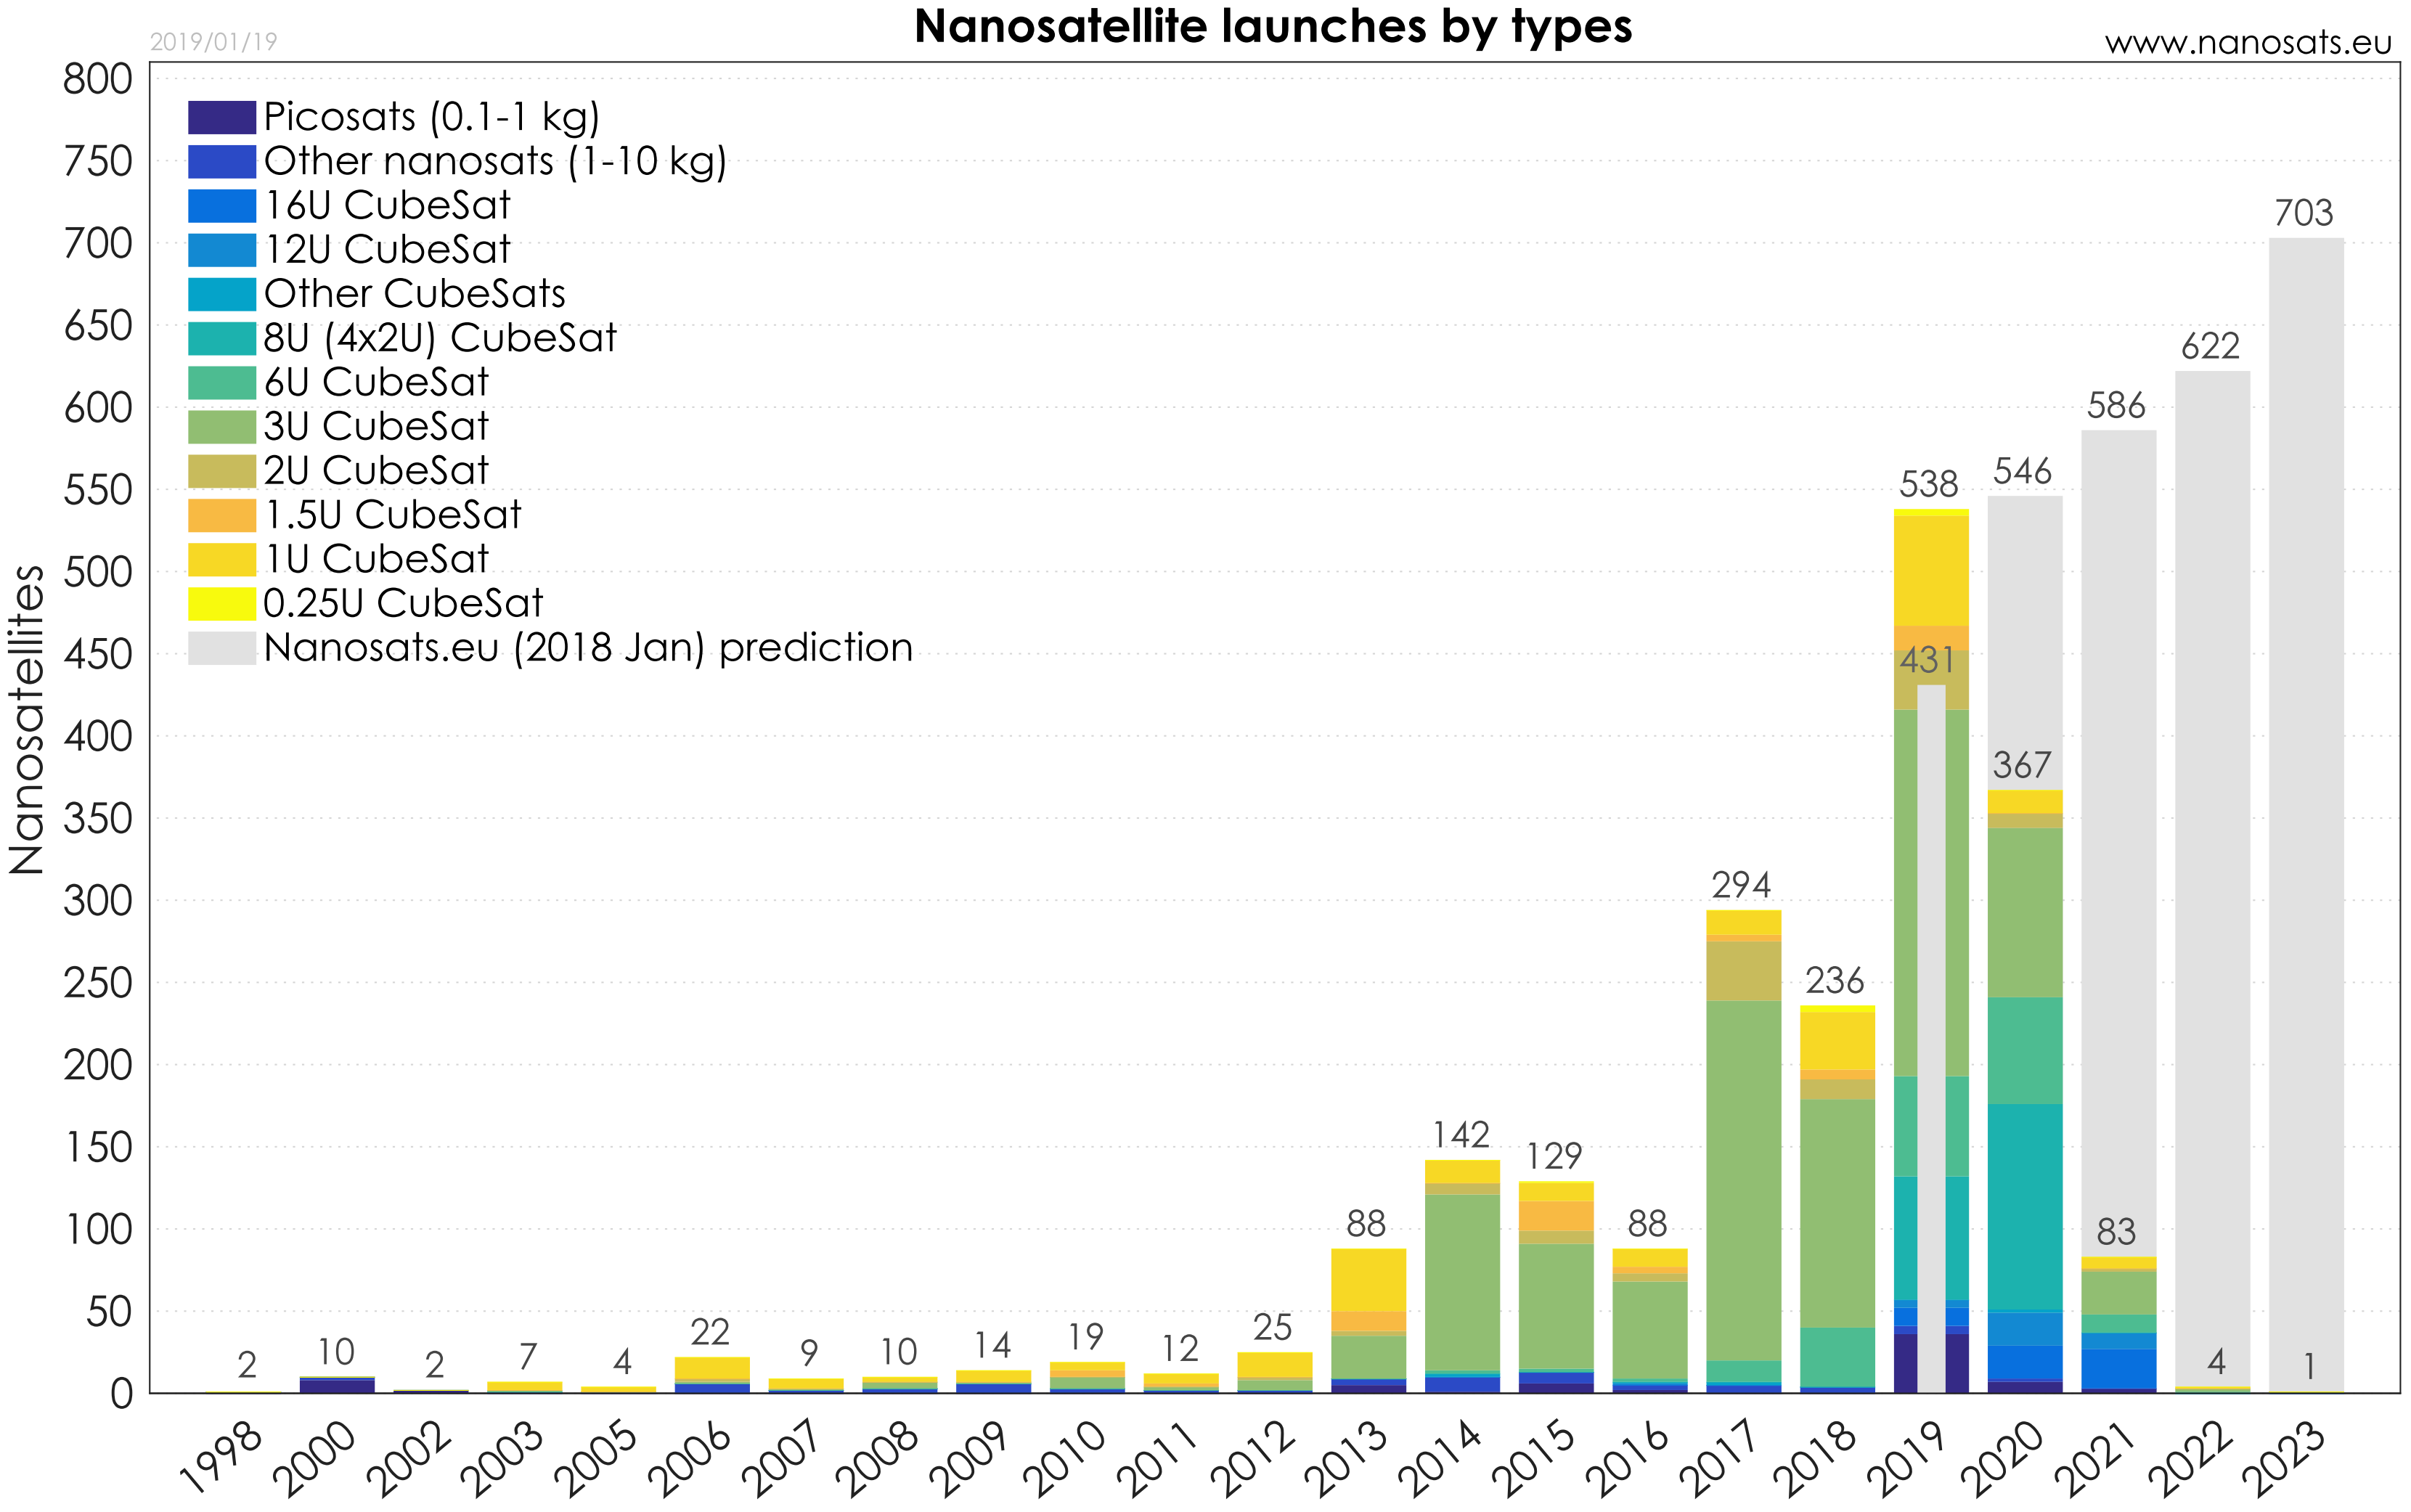
\includegraphics[width=0.80\textwidth]{Nanosats_years_types_2019-01-19_01}
				\caption{Überblick über Nanosatelliten.Missionen von 1998 bis 2023}
				\label{fig:NanosatsTypes}
			\end{figure}

	\newpage
	\subsection{Gestaltungsrichtlinien}
		
	\begin{-}
Für die Gestaltung von CubeSats gelten eine Reihe von Richtlinien. Als kleinste Einheit (1U) wird ein Würfel mit einer Kantenlänge von 10cm und einer zulässigen Masse von maximal 1,33 kg vorgegeben. Für größere Volumen und Massen können mehrere Einheiten von CubeSats verbunden werden. Satelliten mit 1U, 1.5U, 2U, oder 3U können von dem einheitlichen Startmechanismus (P-Pod) in die Erdumlaufbahn ausgelassen werden. Die Kosten von CubeSat Missionen können gering gehalten werden, indem diese als sekundäre Nutzlast bei Raketenstarts mitfliegen. Für größere Satelliten (6U, 12U, 27U) werden andere Startmechanismen benötigt. Die zugelassene Masse wird auf 2 kg/U angehoben. Weitere Vorschriften gelten für die Folgenden Kriterien:
		\begin{itemize}
			\item \textit{Materialien:} 	\\ Alle bei der Konstruktion verwendeten Materialien müssen den Richtlinien der Air Force Space Command Manual \textbf{[AFSPCMAN 91-710 Volume 3]} entsprechen. Außerdem darf der Masseverlust des Satelliten maximal 1\% betragen.
			\item \textit{Energiespeicher:} \\ Der chemische Energiespeicher darf eine Größe von 100 Wh nicht überschreiten. 
			\item \textit{Aktivierungszeitpunkt:} \\ Während der CubeSat im P-POD verstaut ist müssen alle Systeme ausgeschaltet bleiben. Beim Verlassen der Trägerrakete wird der Satellit aktiviert. Erst 30 Minuten später dürfen Bauteile (z.B. Solarpanele, Antennen, etc...) ausgefahren werden. Bevor die ersten Signale generiert oder gesendet werden müssen mindestens 45 Minuten vergangen sein. 
		\end{itemize}
%Allgemein gelten noch weitere Vorschriften für die verwendeten  Materialien, Kommunikationsfähigkeit, gespeicherte Energie und Aktivierungszeitpunkt der Systeme nach Einsatz in die Umlaufbahn. 
Falls ein Entwurf nicht den Vorschriften entspricht, kann bei dem Betreiber der Trägerrakete eine Sondergenehmigung angefragt werden. Nach einer Reihe von Tests entscheidet dieser ob er die Abweichungen akzeptiert, Änderungen vorgenommen werden müssen, oder ein anderer Anbieter gefunden werden muss. 
		\end{-}

			
	\section{Cubesat Subsysteme}
	hier Hauptsächlich das Fazit von max kompakt darstellen und refernzieren
		\subsection{Antrieb - propulsion}
		\subsection{Energie - EPS}
		\subsection{Guidance, navigation and control -GNC ADCS}
		\subsection{Command and data handling}
		\subsection{Communications}
		\subsection{Thermal}
		\subsection{Structure}
				
	\section{RDVDO Mechanismen} das kann ausführlich sein
		\subsection{Docking Strategien}
						\textbf{Roboterarm}
						\textbf{Fangnetz}
						\textbf{Adhäsiv Docken}
						Übersichtstabelle/Graphik: sihe die Quellen die ich am 15.05.2019 gezeigt habe
		\subsection{Bionische Materialien}
						\textbf{Was sind Geckomaterialen}
						\textbf{Bisher getestete Gecko-Materialien}
						\textbf{Bisherige Erfolge}
						\textbf{State of the Art}
						\textbf{Problematik}															% -"- Grundlagen
	\chapter{CubeSat Design}
\hfill\emph{(Florian Czorny, Valentina Dietrich)}

	Für die Realisierung einer ADR-Mission liegt der Fokus zunächst bei dem Entwurf eines geeigneten CubeSats. Infolgedessen wird in diesem Kapitel ein bestehendes Konzept \cite{Lettau.} anhand der Software QuSAD (SQL-Based CubeSat Analyse and Design Tool QuSAD) analysiert und gegebenenfalls optimiert. Zuvor wird ein Einblick in das Programm gegeben und durch eine anschließende Beschreibung des angenommenen Entwurfs erfolgt abschließend die Budgetplanung. Letztlich wird mittels der Budgets eine Auswertung des Designs bezüglich seiner Effizienz durchgeführt. Bei Bedarf werden Verbesserungen in Erwägung gezogen. Demnach kann ein zielführendes Missionsdesign bestimmt und bewertet werden.
		
		\section{QuSAD}
			
			\subsection{Einführung in die Software}
	\hfill\emph{(Valentina Dietrich)}
	
		Die Software QuSAD (SQL-Based CubeSat Analyse and Design Tool) besteht aus einem SQL-Segment und einem MatLab Segment. Die SQL-Datenbank ist die Haupteingabequelle für das Entwerfen eines CubeSats und kategorisiert die CubeSat-Komponenten. Durch die wissenschaftliche Version können die COTS-Komponenten mit vordefinierten Parametern eingepflegt werden. Zusätzlich können auch individuelle Komponenten mit veränderbaren Parametern mittels der Praxisversion hinzugefügt werden. Für das Abrufen der Komponententabelle aus der SQL-Datenbank wird MatLab verwendet. Dies wird durch mehrere grafische Benutzeroberflächen (GUI) realisiert und ermöglicht dem Benutzer eigene Satellitenzusammenstellungen. Neben dem CubeSat Design können Budget-Analysen von Masse, Volumen, Energie, Preis und Verlinkung durch zur Verfügung stehenden Werkzeuge erstellt werden, um folglich eine Optimierung des Entwurfs zu ermöglichen. Für ein vertieftes Verständnis der Software wird auf das QuSAD-Handbuch \cite{Farahvashi.2016} verwiesen. Das Anwendungsspektrum von QuSAD umfasst das Erstellen eines Satelliten, sowie eine Bereitstellung einer Datenbank von Subsystemen für wissenschaftliche und auch lehrende Aspekte. Lehrende Aspekte umfassen den Einsatz der praktischen Version an Universitäten zur Unterstützung und Visualisierung \cite{Farahvashi.2016b}. 
			
			\subsection{Datenbankerweiterung}
			\hfill\emph{(Florian Czorny, Valentina Dietrich)}
			
			Zur Erweiterung der Datenbank wird anfänglich die Auswahl der CubeSat-Komponenten einer ausgewählten Systemzusammenstellung verwendet (siehe \tab{qusadwerte}). Zu den besagten Komponenten werden alle bekannten Werte der Datenbank hinzugefügt. Zudem müssen Recherchen bezüglich weiterer Herstellerangaben durchgeführt werden. Im Fokus liegen dabei alle Parameter die für die Budgetplanungen benötigt werden. Nach der Budgetanalyse, des zusammengestellten Satelliten, wird gegebenenfalls die Optimierung einiger Komponenten vorgenommen und infolgedessen die Datenbank um diese Systeme zusätzlich erweitert. Zur Unterstützung der Ergänzungen wird eine  Datenbank, die von Mitarbeitern des Institutes Raumfahrtsysteme der Technischen Universität Braunschweig erstellt worden ist, verwendet. Überwiegend sind die aufgelisteten Systeme mit einem TRL Wert hinterlegt. Da in vielen Fällen nur erprobte Systeme zum Einsatz kommen, werden Komponenten mit einem TRL Wert von \num{9} mit in die Datenbank hinzugefügt. Zusätzlich sind Internet-Quellenverweise (URL - Uniform Resource Locator) zu den meisten Einträgen vorhanden, über die man häufig direkt oder indirekt auf Datenblätter weitergeleitet wird und an weitere Informationen bezüglich des Subsystems gelangt.
			
			\subsection{Problematik}
			\hfill\emph{(Florian Czorny, Valentina Dietrich)}
			
			Die Datenbankerweiterung und Budgeterstellung führt zu einigen Schwierigkeiten. Bei dem Laden der Datenbank über den SQL Server sind Fehlermeldungen bei MatLab aufgetreten, die nicht direkt behoben werden können. Die Ursache könnte an der Inkompatibilität zwischen den neuen MatLab Versionen und MySQL liegen, da QuSAD mit der MatLab Version R2014 erstellt wurde. Im QuSAD Handbuch wird auf dieses Problem hingewiesen. Infolgedessen wird die Datenbank über MySQL importiert und Lokal darauf zugegriffen. Die Datenbank wird in Mat-File Dateien gespeichert und kann über MatLab aufgerufen werden. Anschließend können die Komponenten in die gespeicherte Datenbank eingepflegt und als Workspace gesichert werden. Durch das Exportieren der neuen Datenbank über MySQL wird der Zugriff künftig bereitgestellt. Besonders problematisch gestaltete sich das einpflegen der Komponenten in die Datenbank. Im Handbuch, sowie den weiteren Dokumenten zur Datenbank wird der Vorgang nicht hinreichend genau beschrieben. Weiterhin gibt es viele, unbekannte Angaben über die hinzugefügten Komponenten. Diese müssen einzeln recherchiert und in seltenen Fällen abgeschätzt werden. Außerdem sind einige URLs nicht mehr Gültig. Bei der Erstellung des Leistungsbudgets muss die im EPS integrierte Batterie zusätzlich angegeben werden, um ein Leistungsbudget erstellen zu können. Die Kapazität der Batterie ist ein entscheidender Parameter für das Budget. 
		
		\section{CubeSat Designanalyse}
				
				\subsection{Angenommenes Design}
				\label{cap:AngenommenesDesign}
				\hfill\emph{(Valentina Dietrich)}
				
				Diese CubeSat Konfiguration orientiert sich an einem entwickelten Design \cite{Lettau.}. Hier wird ein ausführlicher Vergleich und anschließend eine Auswertung der in Betracht gezogenen Subsysteme durchgeführt. Durch den Schwerpunkt auf das GNC-Design erfolgt eine vertiefte Ausarbeitung der Subsysteme Antrieb, Leistung und relative Navigation. Die weiteren Systeme werden stark vereinfacht und nur in Bezug auf ihren Beitrag zum Gesamtbudget weitgehend abgedeckt \cite{Lettau.}. 
				
				Daran angeknüpft wird vorweg auf die betrachteten Anforderungen, die beim Entwicklungsprozess entscheidend sind, eingegangen. Anschließend wird ein Ausblick auf die Struktur, den Antrieb, das Power Management and Distribution System (PMAD-System) und das Solarpanel gegeben. Für ein vertieften Einblick in die weiteren Subsysteme wird auf die Masterarbeit von Max Lettau verwiesen \cite{Lettau.}.

				
				Bei den Anforderungen an die Mission knüpft die Konzeptplanung an der SpaceX-Starlink Konstellation an. Davon abgeleitet wird für die Umlaufbahnparamter wie folgt ausgegangen. Es wird der für die Mission ungünstigste Fall betrachtet, der bei einem Beta-Winkel $\beta$ von 0\textdegree, einer Bahnhöhe von \SI{1150}{\kilo\metre} und einer Missionsdauer von \num{10} Jahren vorliegt. Darauf aufbauend wurde das CubeSat Design entwickelt \cite{Lettau.}.
				
				Bei der Primärstruktur wird von einem \SI{27}{\unit} CubeSat mit einer zugelassen maximalen Masse von \SI{50}{\kilogram} und einer Gesamtabmessung von \SI{34 x 35 x 36}{\centi\metre} ausgegangen (siehe \abb{fig:27U}) \cite{Lettau.}. 
				
				\begin{figure}[H]
					\centering
						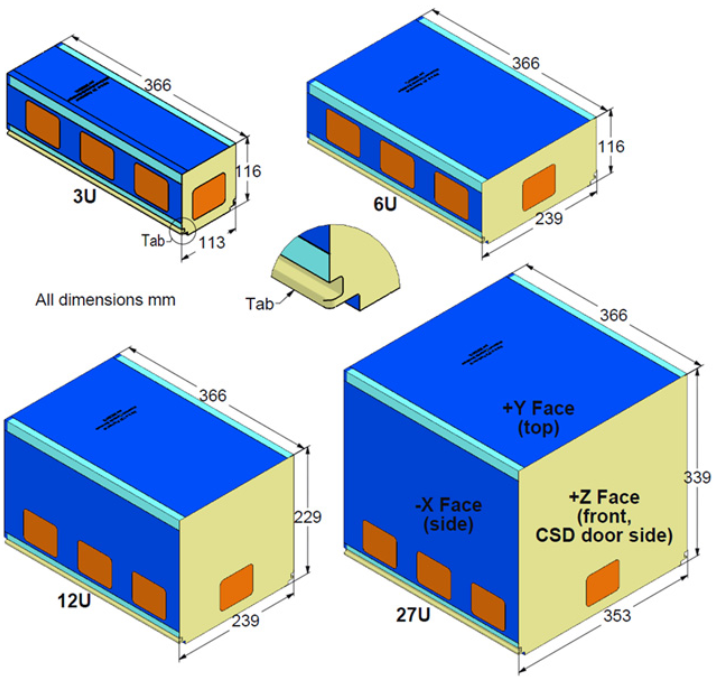
\includegraphics[width=0.60\textwidth]{27U}
					\caption{CubeSat-Größen gemäß der Planetary Systems Corporation \cite{Lettau.}}
					\label{fig:27U}
				\end{figure}
				
				Das Hauptantriebssystem ist der BHT-200 und wird mit dem Treibstoff Iod betrieben. Hier handelt es sich um einen elektrischen Antrieb mit einem TRL-Wert von \num{8} und einem leistungspezifischen Schub von \SI{65}{\micro\newton\watt}. Durch das geringe Volumen von \SI{3}{\unit} und der Verwendung von leichten Materialien für die Tankwände bewährt sich Iod als Treibstoff. 
				
Als weiteres Triebwerk wird das chemische Triebwerk Marotta verwendet. Dies dient zur Ausführung von Rendevouz und Docking. Durch die Auslegung der Kaltgaspakete für sehr kleine Satelliten (< \SI{6}{\unit}) weisen sie sehr geringe Schübe auf und erreichen nicht den Schub von \SI{0,23}{\newton}. Trotz dessen werden \num{24} Marotta Triebwerke verwendet, um eine 6-DoF-Manövrierfähigkeit zu ermöglichen. Sie weisen im Vergleich zu anderen Kaltgastriebwerken einen hohen $I_{sp}$ Wert von \SI{65}{\second} auf. Die Anordnung der Marotta Triebwerken ist der \abb{fig:marotta} zu entnehmen. Dieses Triebwerk wird mit Stickstoff angetrieben und benötigt bei \num{40}\% Sicherheit und der Annahme einer Stabilisierung von einer Sekunde alle \num{10} Orbits eine Gesamttreibstoffmasse von \SI{2,12}{\kilo\gram} \cite{Lettau.}.
				
				\begin{figure}[H]
					\centering
						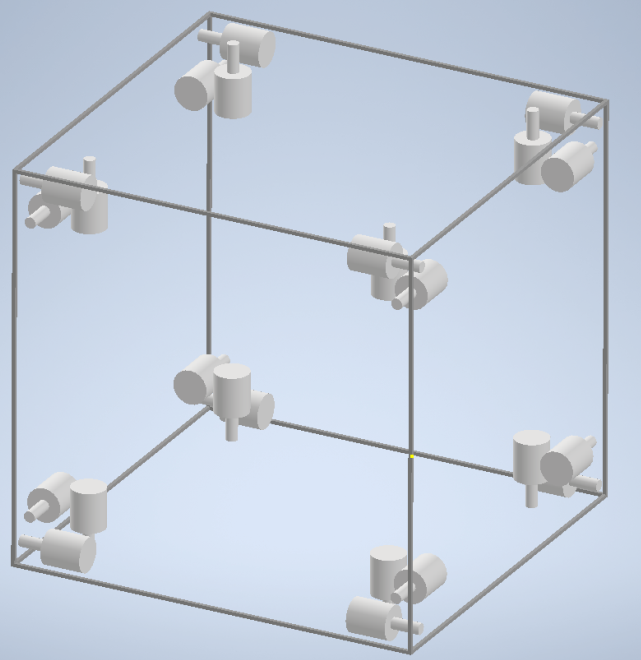
\includegraphics[width=0.30\textwidth]{Marotta}
						\caption{Anordnung der RCS-Triebwerke \cite{Lettau.}}
						\label{fig:marotta}
				\end{figure}
				
				Viele Unternehmen bieten kundenspezifische Lösungen an. Dies wird auch von dem Unternehmen Blue Canyon Technologies für das Solarmodul \SI{6}{\unit}-H triple deployable solar array angeboten. Da es sich um eine zweiflügelige Konfiguration mit einer Grundfläche von \SI{6}{\unit} pro Flügel handelt, wird sie auf eine Grundfläche von \SI{9}{\unit} hoch skaliert, sodass sie auf den \SI{27}{\unit} CubeSat angewendet werden kann. Weiterhin wird von einer dreiflügeligen Konstellation ausgegangen. Die Vergrößerung der Solaranlage sorgt für eine Steigerung der Nennleistung um \num{50}\%. Weiterhin wird ein Solarpanel auf die obere Grundfläche des CubeSats platziert. Mit allen sieben Solarpanelen erreicht der CubeSat eine Nennleistung von \SI{202}{\watt}. In der \abb{fig:solarpanel} ist eine vereinfachte Darstellung von der Solaranlage zu sehen \cite{Lettau.}.
				
				\begin{figure}[H]
					\centering
						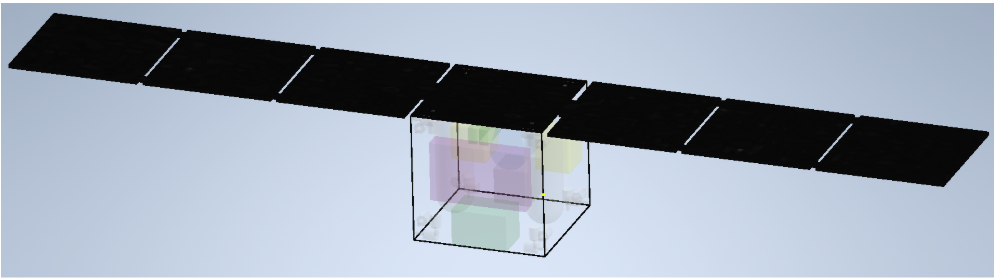
\includegraphics[width=0.60\textwidth]{graphics/Solarpanel.PNG}
						\caption{Vereinfachte Darstellung von der Solarkonfiguration \cite{Lettau.}}
						\label{fig:solarpanel}
				\end{figure}
				
				Bei dem Power Management and Distribution System (PMAD-System) ist das NanoAvionics EPS, mit einem TRL von \num{9}, dass geeignetste PMAD-System. Diese Variante besticht durch das mitgelieferte externe Batteriepacket. Die EPS Variante liefert eine Leistung von \SI{175}{\watt} und eine Kapazität von \SI{161}{\watt\hour}. Zudem kann die Batterie skaliert werden, um die Leistungsabgabe zu erhöhen. Unter der Annahme, dass eine relative Navigation von ca. \SI{5}{\kilo\metre} bis zum Andocken erforderlich ist und ein einziger Sensor dies nicht abdecken kann, sind mehrere miteinander kompatible Sensoren erforderlich. Als Referenz wird die Mission e.Deorbit-Mission aufgrund von Ähnlichkeiten des Missionsprofils gewählt \cite{Lettau.}.  

				Einen Übersicht über die Komponenten des angenommen Designs ist in der \tab{tab:cubesatdesign} zusehen. Hier werden die Subsysteme mit den dazugehörigen Produkten und deren Mengenangabe aufgelistet. Diese Einordnung orientiert sich an der Struktur der QuSAD Datenbank.
				\begin{table}[H]
				\centering
\begin{tabular}{|l|l|c|}
\hline
\multicolumn{1}{|c|}{Subsystem} & \multicolumn{1}{c|}{Produkt}    	            & Anzahl \\ \hline
Antenne                         & IQW S-Band Dual Patch Antenna                 & 2      \\ \hline
                                & SkyFox Labs piPATCH-MAX (GNSS)                & 2      \\ \hline
Kontroll Board                  & SSTL OBC750 LEO Flight Computer               & 1      \\ \hline
EPS                             & NanoAvionics EPS                              & 1      \\ \hline
Nutzlast \& Verschiedenes       & Vision-based LiDAR Sensor                     & 1      \\ \hline
                                & Crystalspace CAM1U 5 MP (RNS)                 & 2      \\ \hline
                                & Gecko based                                   & 1      \\ \hline
Antrieb                         & Iodine tank                                   & 1      \\ \hline
                                & Nitrogen tank                                 & 1      \\ \hline
                                & Busek BHT-200 Thruster (electric)             & 1      \\ \hline
                                & Marotta Micro-Thruster (chemical)             & 24     \\ \hline
Solar Panel                     & Top/Bottom BCT 9U                             & 1      \\ \hline
                                & BCT 9U Tripple Wing Solar Array Custom (Side) & 1      \\ \hline
                                & BCT SADA Gimbal System                        & 1      \\ \hline
Transceiver                     & IQW Slink-Phy S-Band Transceiver              & 1      \\ \hline
Struktur                        & 27U NanoAvionics Standard Structure (s)       & 1      \\ \hline
Tracker und Sensor               & TY-Space PST3                                 & 2      \\ \hline
                                & NSS Fine Sun Sensor NFSS-411                  & 4      \\ \hline
                                & Sensonor STIM300                              & 1      \\ \hline
                                & SSTL SGR-Ligo                                 & 1      \\ \hline
\end{tabular}
\caption{Angenommenes Design \cite{Lettau.}}
\label{tab:cubesatdesign}
\end{table}
	
						%Hier die Varainte von Max nehmen und kurz beschreiben
				\subsection{Budgetplanung}
				\hfill\emph{(Florian Czorny)}
				
Im folgenden Kapitel wird auf die mittels QuSAD erstellten Budgets für Masse, Volumen und Leistung eingegangen. In QuSAD werden Komponenten in Kategorien eingeteilt. Die Budgets werden mit diesen Kategorien erstellt. Eine Tabelle mit allen Kategorien und den dazugehörigen Komponenten ist in der \tab{tab:cubesatdesign} zu finden. Die Batterie ist im EPS Board integriert und taucht deshalb im Massen- und Volumenbudget nicht auf. Da QuSAD in der Kategorie EPS keinen Eintrag über speicherbare Energie zulässt, wurde die Batterie nur für das Leistungsbudget hinzugefügt. Des Weiteren ist zu beachten, dass die Komponenten in den unterschiedlichen Budgets keine einheitliche Farbgebung aufweisen. Einbauvorrichtungen wurden in QuSAD nicht berücksichtigt. Die Abweichungen in den Budgets durch das  zusätzliche Gewicht und Volumen sind davon abhängig, inwiefern die Herstellerangaben den Einbau berücksichtigen.

						\subsubsection{Massenbudget}
Das Massenbudget \abb{fig:masse} zeigt die aktuelle Massenverteilung des Designs an. Die maximal verfügbare Masse ist über eine Angabe in der Strukturkomponente begrenzt. Diese beinhaltet einen Wert für die maximale Gesamtmasse. Die maximale Gesamtmasse des CubeSats wurde mit \SI{50}{\kilogram} angenommen. Das aktuelle Design beansprucht circa \num{57}\% der möglichen Gesamtmasse (\SI{28,5}{\kilogram}). Den größten Teil macht dabei die Antriebsanlage aus. Es gilt zu beachten, dass dieses Budget die Startmasse des CubeSats widerspiegelt. Nach Beginn der Mission ändert sich die Massenverteilung aufgrund des Treibstoffverbrauchs.
										%\begin{figure}[H]
											%\centering
											%\scalebox{0.5}{
												%% This file was created by matlab2tikz.
%
%The latest updates can be retrieved from
%  http://www.mathworks.com/matlabcentral/fileexchange/22022-matlab2tikz-matlab2tikz
%where you can also make suggestions and rate matlab2tikz.
%
\definecolor{mycolor1}{rgb}{0.24220,0.15040,0.66030}%
\definecolor{mycolor2}{rgb}{0.28033,0.27823,0.92210}%
\definecolor{mycolor3}{rgb}{0.24403,0.43583,0.99883}%
\definecolor{mycolor4}{rgb}{0.15400,0.59020,0.92180}%
\definecolor{mycolor5}{rgb}{0.02967,0.70817,0.81633}%
\definecolor{mycolor6}{rgb}{0.19377,0.77577,0.62510}%
\definecolor{mycolor7}{rgb}{0.50440,0.79930,0.34800}%
\definecolor{mycolor8}{rgb}{0.86343,0.74060,0.15963}%
\definecolor{mycolor9}{rgb}{0.98920,0.81357,0.18853}%
\definecolor{mycolor10}{rgb}{0.64706,0.64706,0.64706}%
%
\begin{tikzpicture}

\begin{axis}[%
width=8.116in,
height=8.116in,
at={(4.887in,1.095in)},
scale only axis,
xmin=-1.2,
xmax=1.2,
ymin=-1.2,
ymax=1.2,
axis line style={draw=none},
ticks=none,
axis x line*=bottom,
axis y line*=left,
legend style={at={(1.03,1)}, anchor=north west, legend cell align=left, align=left, draw=white!15!black}
]

\addplot[area legend, draw=black, fill=mycolor1]
table[row sep=crcr] $};

\addplot[area legend, draw=black, fill=mycolor2]
table[row sep=crcr] ;

\addplot[area legend, draw=black, fill=mycolor3]
table[row sep=crcr] ;

\addplot[area legend, draw=black, fill=mycolor4]
table[row sep=crcr] {%
x	y\\
-0.064205999219058	0.0766654398297064\\
-0.489757869497587	0.981599473725242\\
-0.54083703763559	0.955768876984845\\
-0.590354618956384	0.927058072646164\\
-0.638148378951558	0.895561125950347\\
-0.684061730870485	0.861381230379937\\
-0.727944248745675	0.824630369565949\\
-0.769652160233538	0.785428950395771\\
-0.809048817655885	0.743905408523941\\
-0.84600514569887	0.700195787578264\\
-0.880400064302586	0.65444329343992\\
-0.064205999219058	0.0766654398297064\\
}--cycle;
\addlegendentry{Miscellaneous\&Payload}

\node[above left, align=right]
at (axis cs:-0.722,0.886) {8\%};

\addplot[area legend, draw=black, fill=mycolor5]
table[row sep=crcr] {%
x	y\\
-0.0935310707482601	-0.0353827472743986\\
-0.909725135831788	0.542395106335816\\
-0.943484459046369	0.491475144116216\\
-0.974071301952834	0.438588666663399\\
-1.00137149810612	0.383933074576735\\
-1.02528314858343	0.327712371736916\\
-1.04571700232544	0.270136403854455\\
-1.06259678926899	0.211420075213331\\
-1.07585950502768	0.151782546533346\\
-1.08545564605798	0.0914464169451898\\
-1.09134939443282	0.0306368931315142\\
-1.09351875153334	-0.0304190512647726\\
-1.0919556201594	-0.0914935228274465\\
-1.08666583475271	-0.152358558986996\\
-1.07766913961958	-0.212786978898768\\
-1.06499911523457	-0.272553231403299\\
-1.04870305290028	-0.33143423690379\\
-1.02884177823086	-0.389210220018385\\
-1.00548942411837	-0.445665529899358\\
-0.978733154029164	-0.500589445157337\\
-0.948672836663279	-0.553776960386141\\
-0.915420673191051	-0.605029551352532\\
-0.879100778458387	-0.654155915994751\\
-0.839848717723829	-0.700972688464055\\
-0.79781100065655	-0.745305123544068\\
-0.753144534483973	-0.786987748893318\\
-0.706016038330127	-0.825864982676459\\
-0.656601420930786	-0.861791714278828\\
-0.605085124048037	-0.894633845936815\\
-0.55165943403506	-0.924268793262386\\
-0.496523764120683	-0.950585942793536\\
-0.439883910092637	-0.973487064862847\\
-0.38195128215768	-0.992886680243107\\
-0.322942115845731	-1.00871237920147\\
-0.0935310707482601	-0.0353827472743986\\
}--cycle;
\addlegendentry{Propulsion}

\node[left, align=right]
at (axis cs:-1.093,-0.41) {31\%};

\addplot[area legend, draw=black, fill=mycolor6]
table[row sep=crcr] ;

\addplot[area legend, draw=black, fill=mycolor7]
table[row sep=crcr] ;

\addplot[area legend, draw=black, fill=mycolor8]
table[row sep=crcr] ;

\addplot[area legend, draw=black, fill=mycolor9]
table[row sep=crcr] $};

\addplot[area legend, draw=black, fill=mycolor10]
table[row sep=crcr] {%
x	y\\
0.097782419365908	0.0209427424887404\\
0.507348825107156	-0.891337564921321\\
0.562918328086794	-0.864296539523979\\
0.616711390182738	-0.833874620020343\\
0.66852256564682	-0.800187993401254\\
0.71815397792597	-0.763365315183601\\
0.765416075389717	-0.723547218050878\\
0.810128355263262	-0.680885774750708\\
0.852120053001271	-0.635543917300627\\
0.891230794469563	-0.587694814720284\\
0.927311208443872	-0.537521211666625\\
0.960223497086443	-0.485214730497921\\
0.989841962221698	-0.430975139432211\\
1.01605348540105	-0.375009589595171\\
1.03875795992336	-0.31753182387129\\
1.05786867316115	-0.258761360579881\\
1.07331263773228	-0.198922655093637\\
1.08503087025243	-0.138244242601652\\
1.09297861660361	-0.0769578652908584\\
1.09712552285855	-0.0152975872793493\\
1.09745575120795	0.0465010993181915\\
1.09396804044811	0.108202173778847\\
1.08667571079761	0.169569988178679\\
1.07560661302499	0.230370167376145\\
1.06080302208142	0.290370504134527\\
1.04232147564477	0.349341845964723\\
1.0202325581917	0.407058970301397\\
0.994620631422304	0.463301444669999\\
0.96558351206707	0.517854468559548\\
0.933232098306511	0.57050969378589\\
0.897689946230302	0.621066020212317\\
0.859092797953509	0.669330363788533\\
0.817588063192105	0.715118393974699\\
0.773334256277737	0.758255237734178\\
0.726500390761906	0.798576147406316\\
0.677265333921642	0.835927129908519\\
0.625817123631992	0.870165534864587\\
0.572352250214251	0.901160599413136\\
0.517074906002747	0.928793947615382\\
0.460196205496184	0.952960042554956\\
0.401933379071958	0.973566589403087\\
0.34250894334278	0.990534887909792\\
0.282149851324192	1.00380013297482\\
0.221086625658615	1.01331166215044\\
0.159552478206344	1.01903314913077\\
0.0977824193659083	1.02094274248874\\
0.097782419365908	0.0209427424887404\\
}--cycle;
\addlegendentry{Margin}

\node[right, align=left]
at (axis cs:1.13,0.222) {43\%};
\end{axis}
\end{tikzpicture}%
												%}
											%\caption{Massenbudget für das angenommene Design}
											%\label{fig:masse}
										%\end{figure}
										
										%\begin{figure}[H]
											%\centering
												%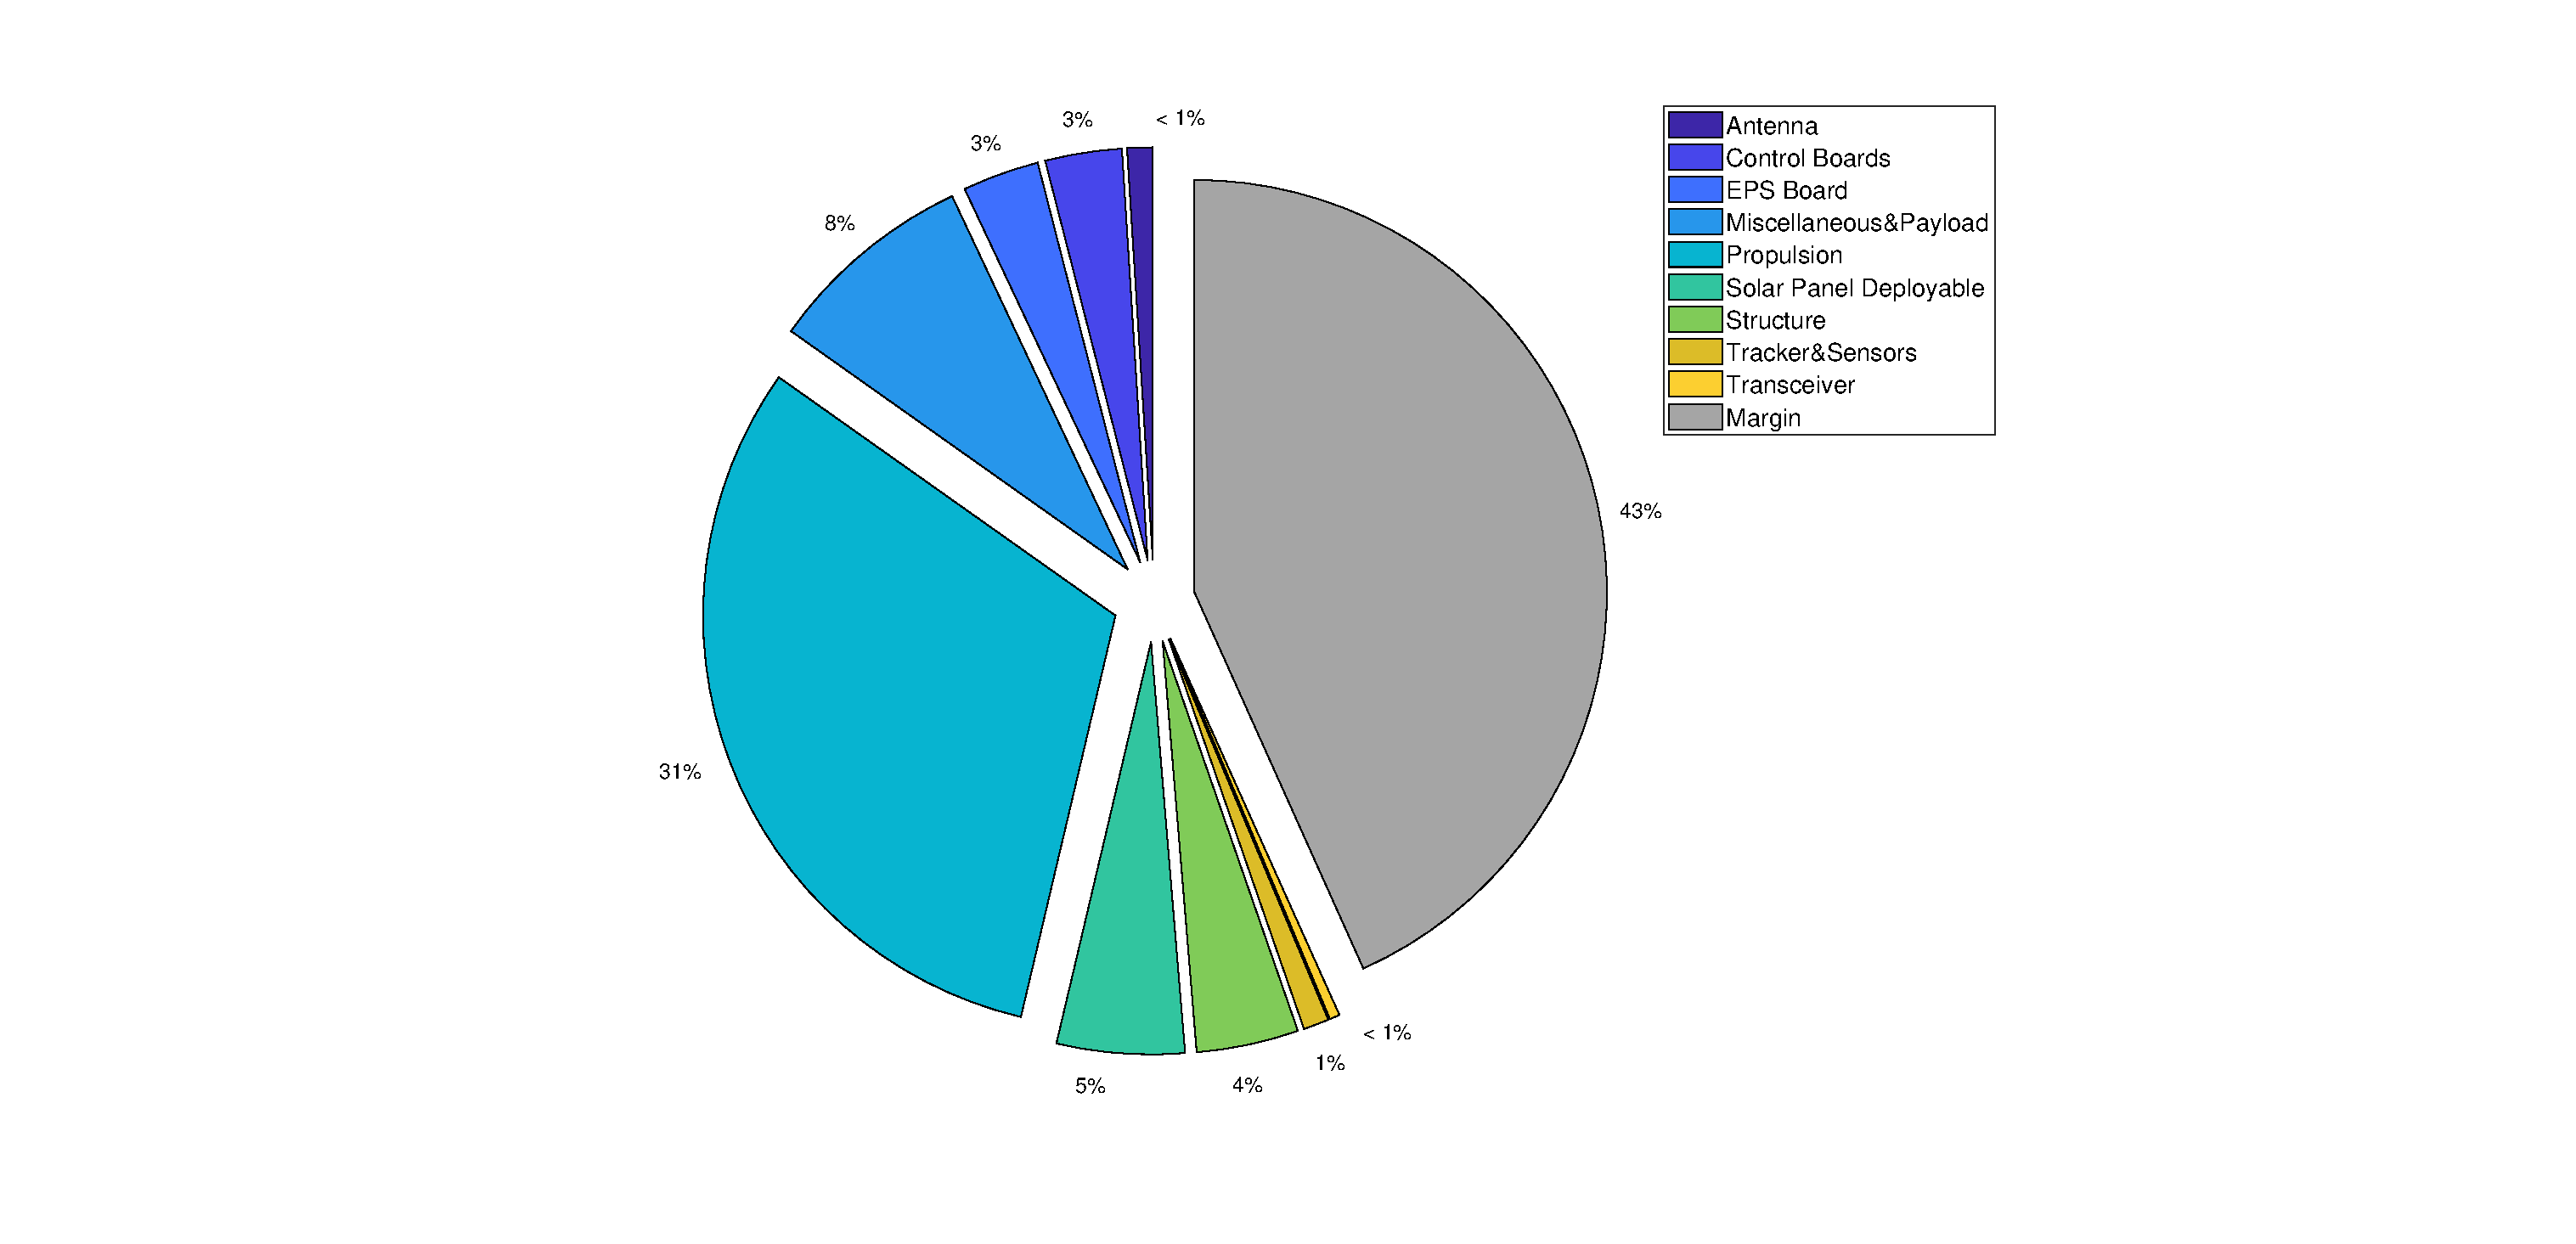
\includegraphics[width=1.50\textwidth]{./Budget/masse.eps}
											%\caption{Massenbudget für das angenommene Design}
											%\label{fig:masse}
										%\end{figure}
								
											\begin{figure}[H]
											\centering
												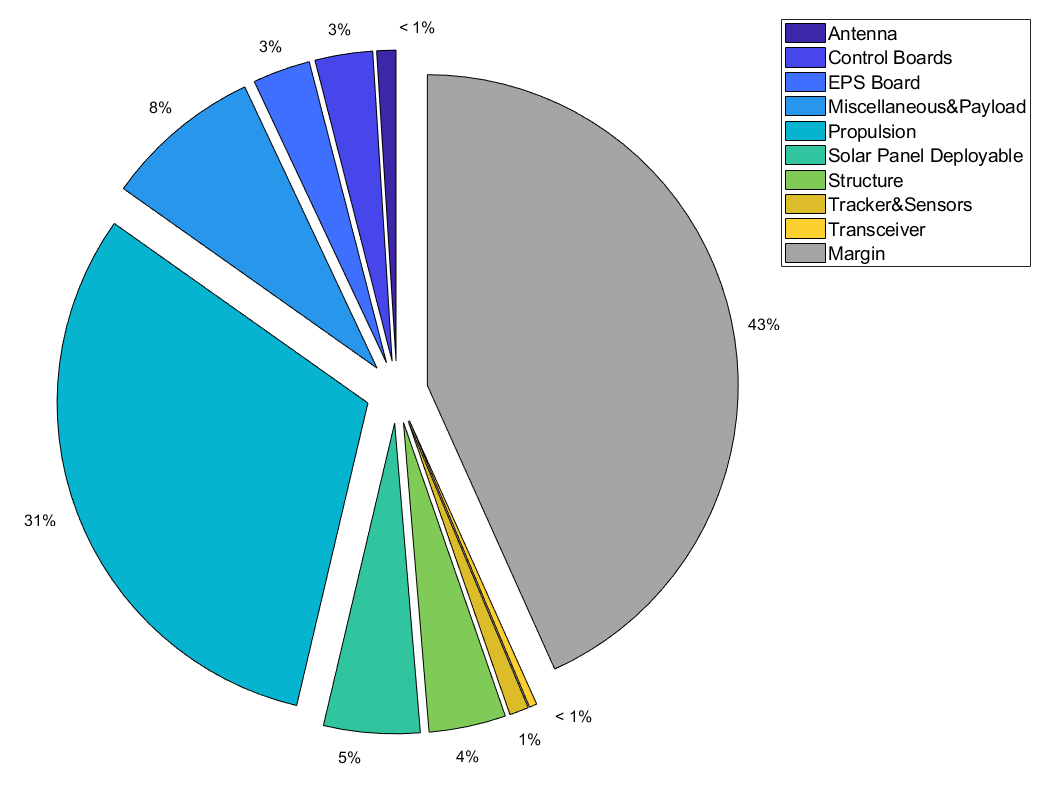
\includegraphics[width=0.90\textwidth]{./Budget/masse_neu}
											\caption{Massenbudget für das angenommene Design}
											\label{fig:masse}
										\end{figure}
										
						\subsubsection{Volumenbudget}
Das Volumenbudget \abb{fig:volume} gibt einen strukturierten Überblick über die aktuelle Volumenverteilung der ausgewählten Konfiguration, beziehungsweise des Profils in QuSAD. Das maximale verfügbare Volumen bemisst sich an der im Profil befindlichen Strukturkomponente, die über eine Volumenangabe verfügt. Es wurde von einem \SI{27}{\unit} CubeSat mit den Kantenlängen\\ \SI{30 x 30 x 30}{\centi\metre} ausgegangen. Das verfügbare Gesamtvolumen ist bei dieser Annahme im Gegensatz zur Masse jedoch zu circa \num{97}\% ausgelastet. Es fällt auf, dass nahezu alle Kategorien einen größeren Volumenanteil als Massenanteil aufweisen. Das größte Volumen nimmt, ähnlich wie beim Massenbudget die Antriebsanlage ein. Sie macht jedoch der Treibstofftanks über die Hälfte des Gesamtvolumens aus. Es sollte beachtet werden, dass aufgrund des geringen Freiraums kaum Sicherheiten möglich sind.
										
										%\begin{figure}[H]
											%\centering
												%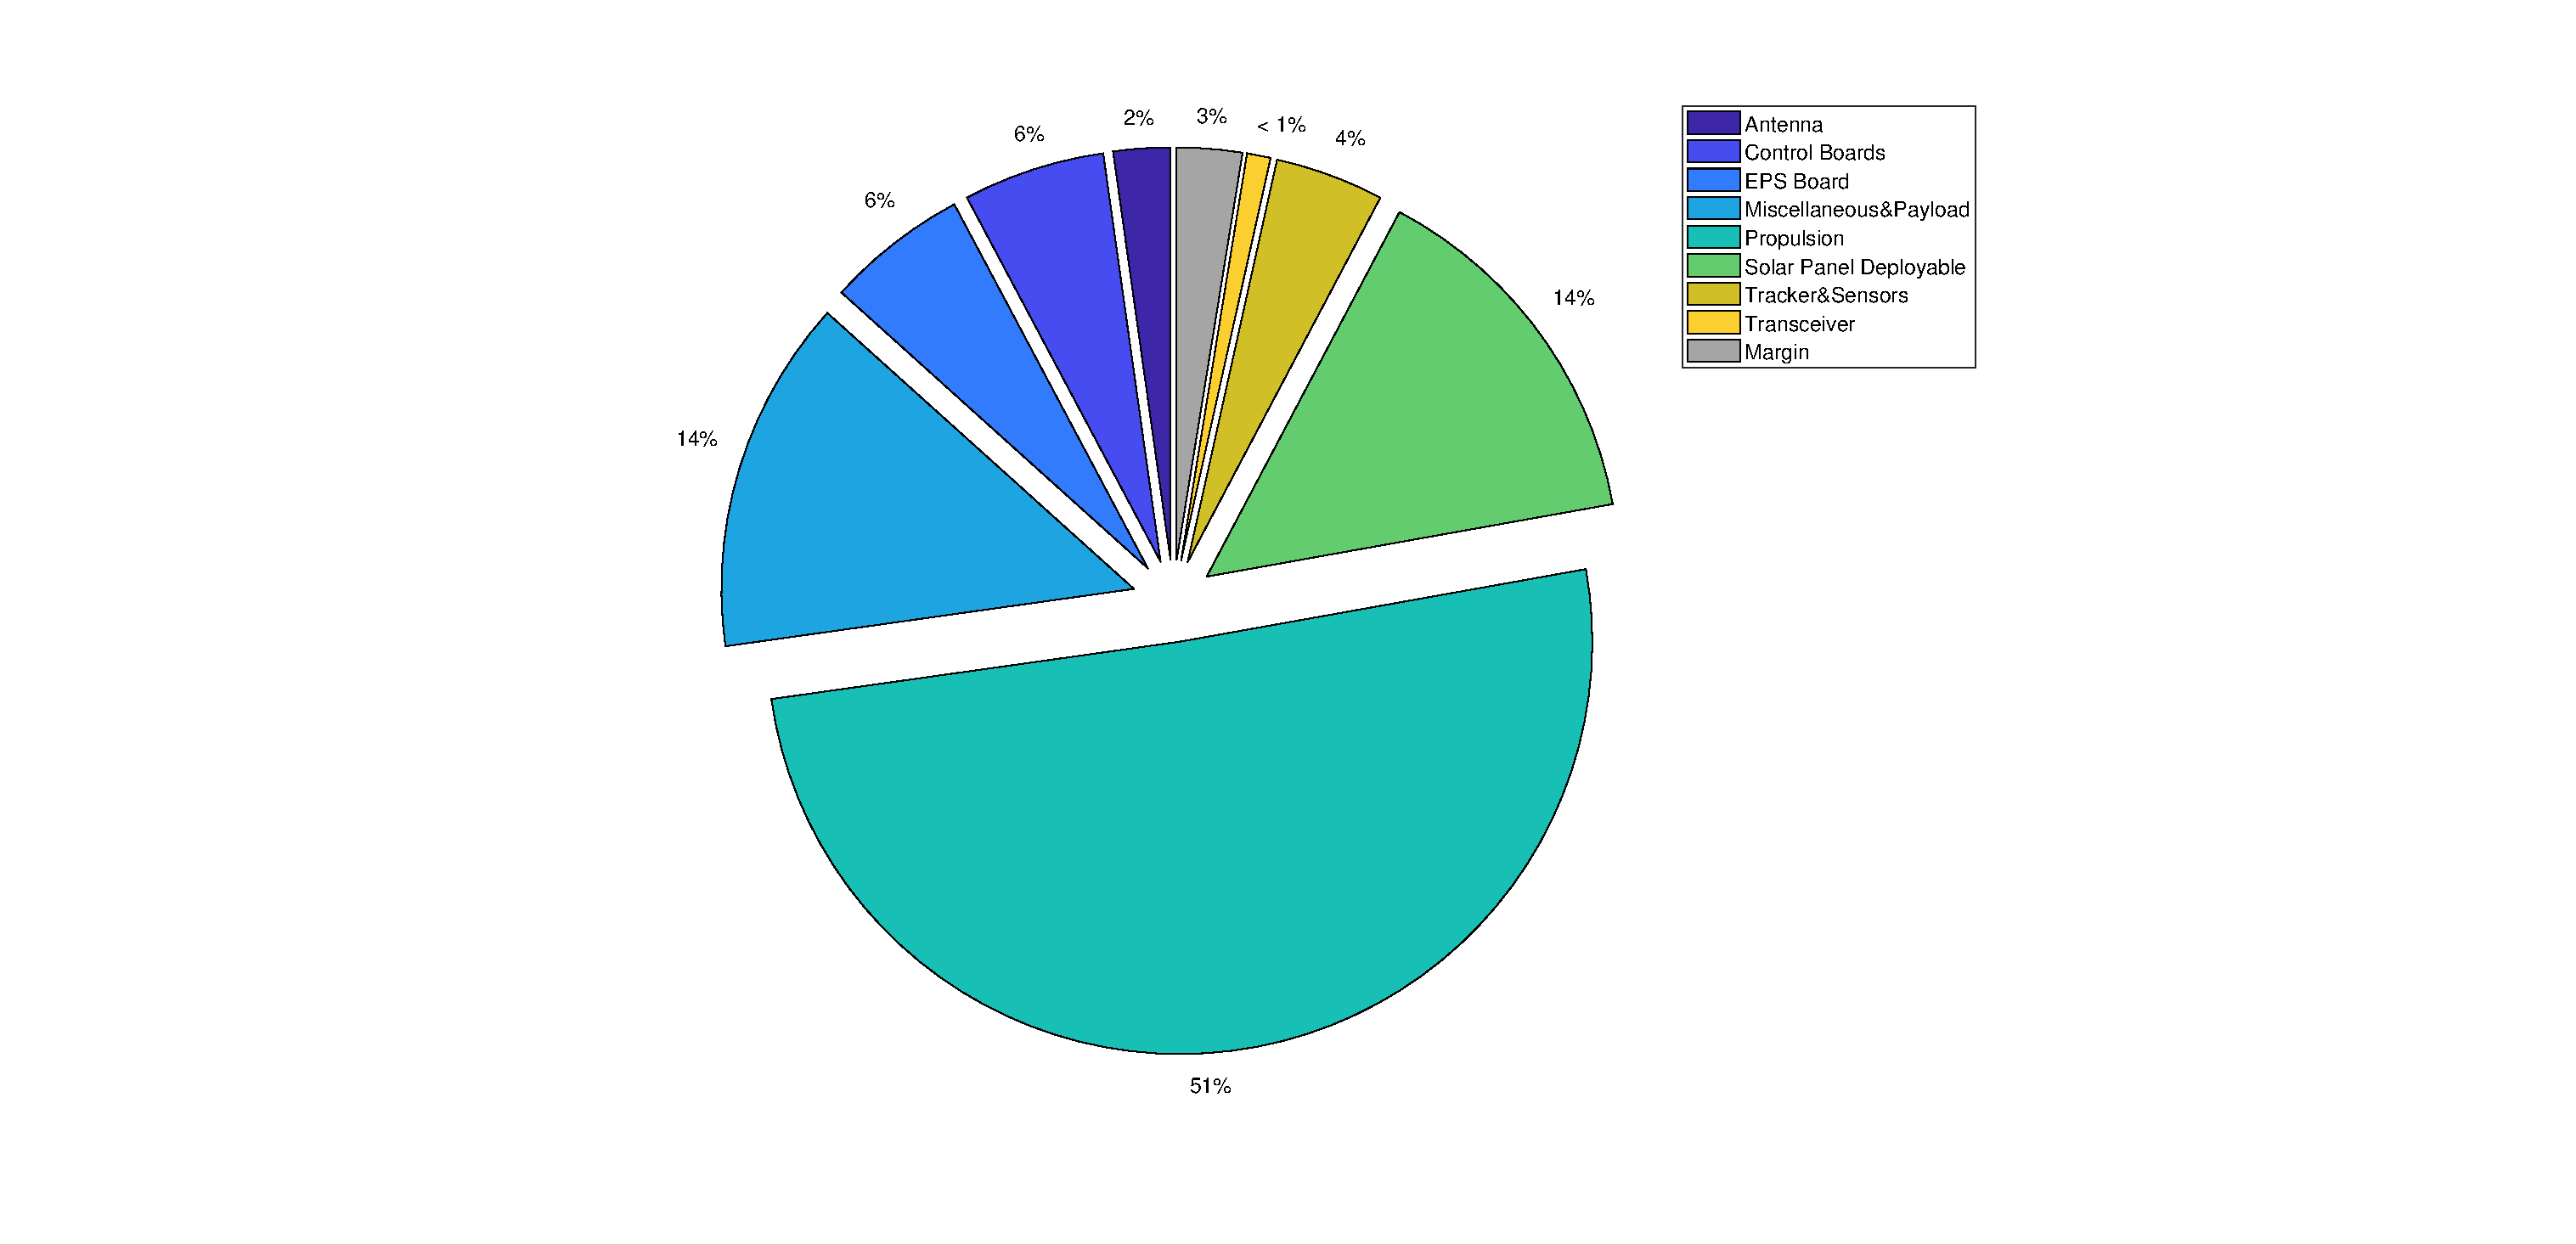
\includegraphics[width=1.50\textwidth]{./Budget/volumen.eps}
											%\caption{Volumenbudget für das angenommene Design}
											%\label{fig:volume}
										%\end{figure}
										%
										\begin{figure}[H]
											\centering
												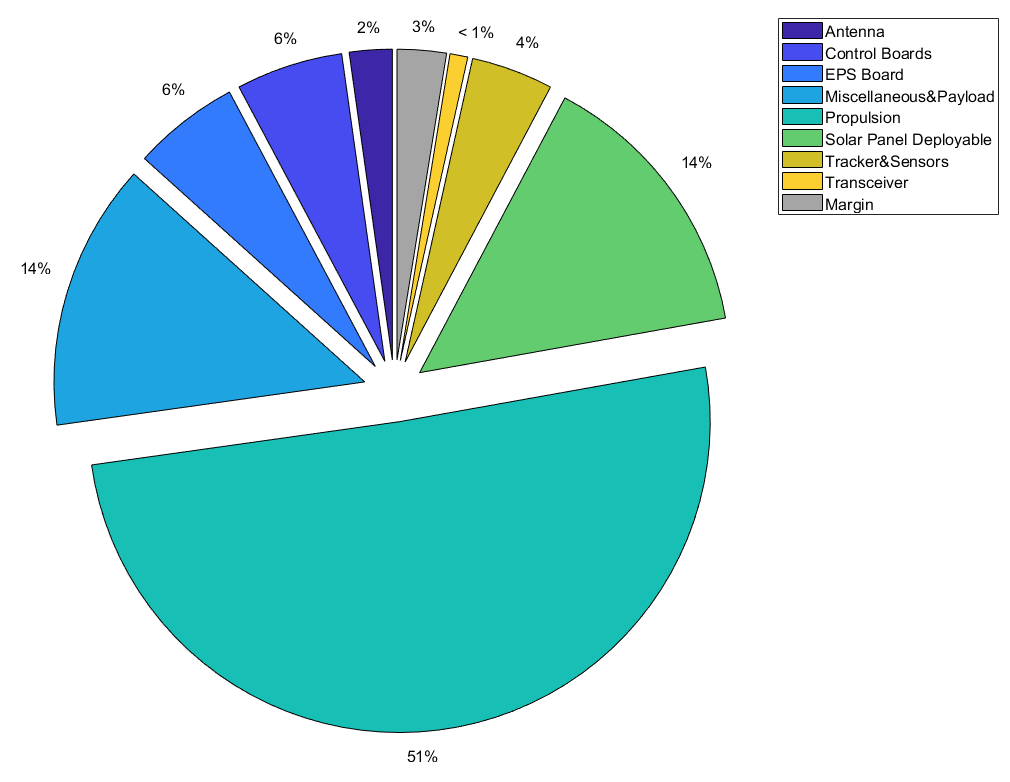
\includegraphics[width=0.90\textwidth]{./Budget/volumen_neu}
											\caption{Volumenbudget für das angenommene Design}
											\label{fig:volume}
										\end{figure}
								
						\subsubsection{Leistungsbudget}
Das Leistungsbudget \abb{fig:power} gibt einen Überblick über den Verbrauch der verschiedenen Komponenten. Es gibt die Entladung der Batterie auf der Schattenseite der Erde wieder (Req. Battery Power) und wie in den anderen Budgets die Spanne zur Systemuntauglichkeit (Margin). Der Antrieb nimmt mit \num{32}\% insgesamt den größten Anteil des Energieverbrauchs ein.
										%\begin{figure}[H]
											%\centering
												%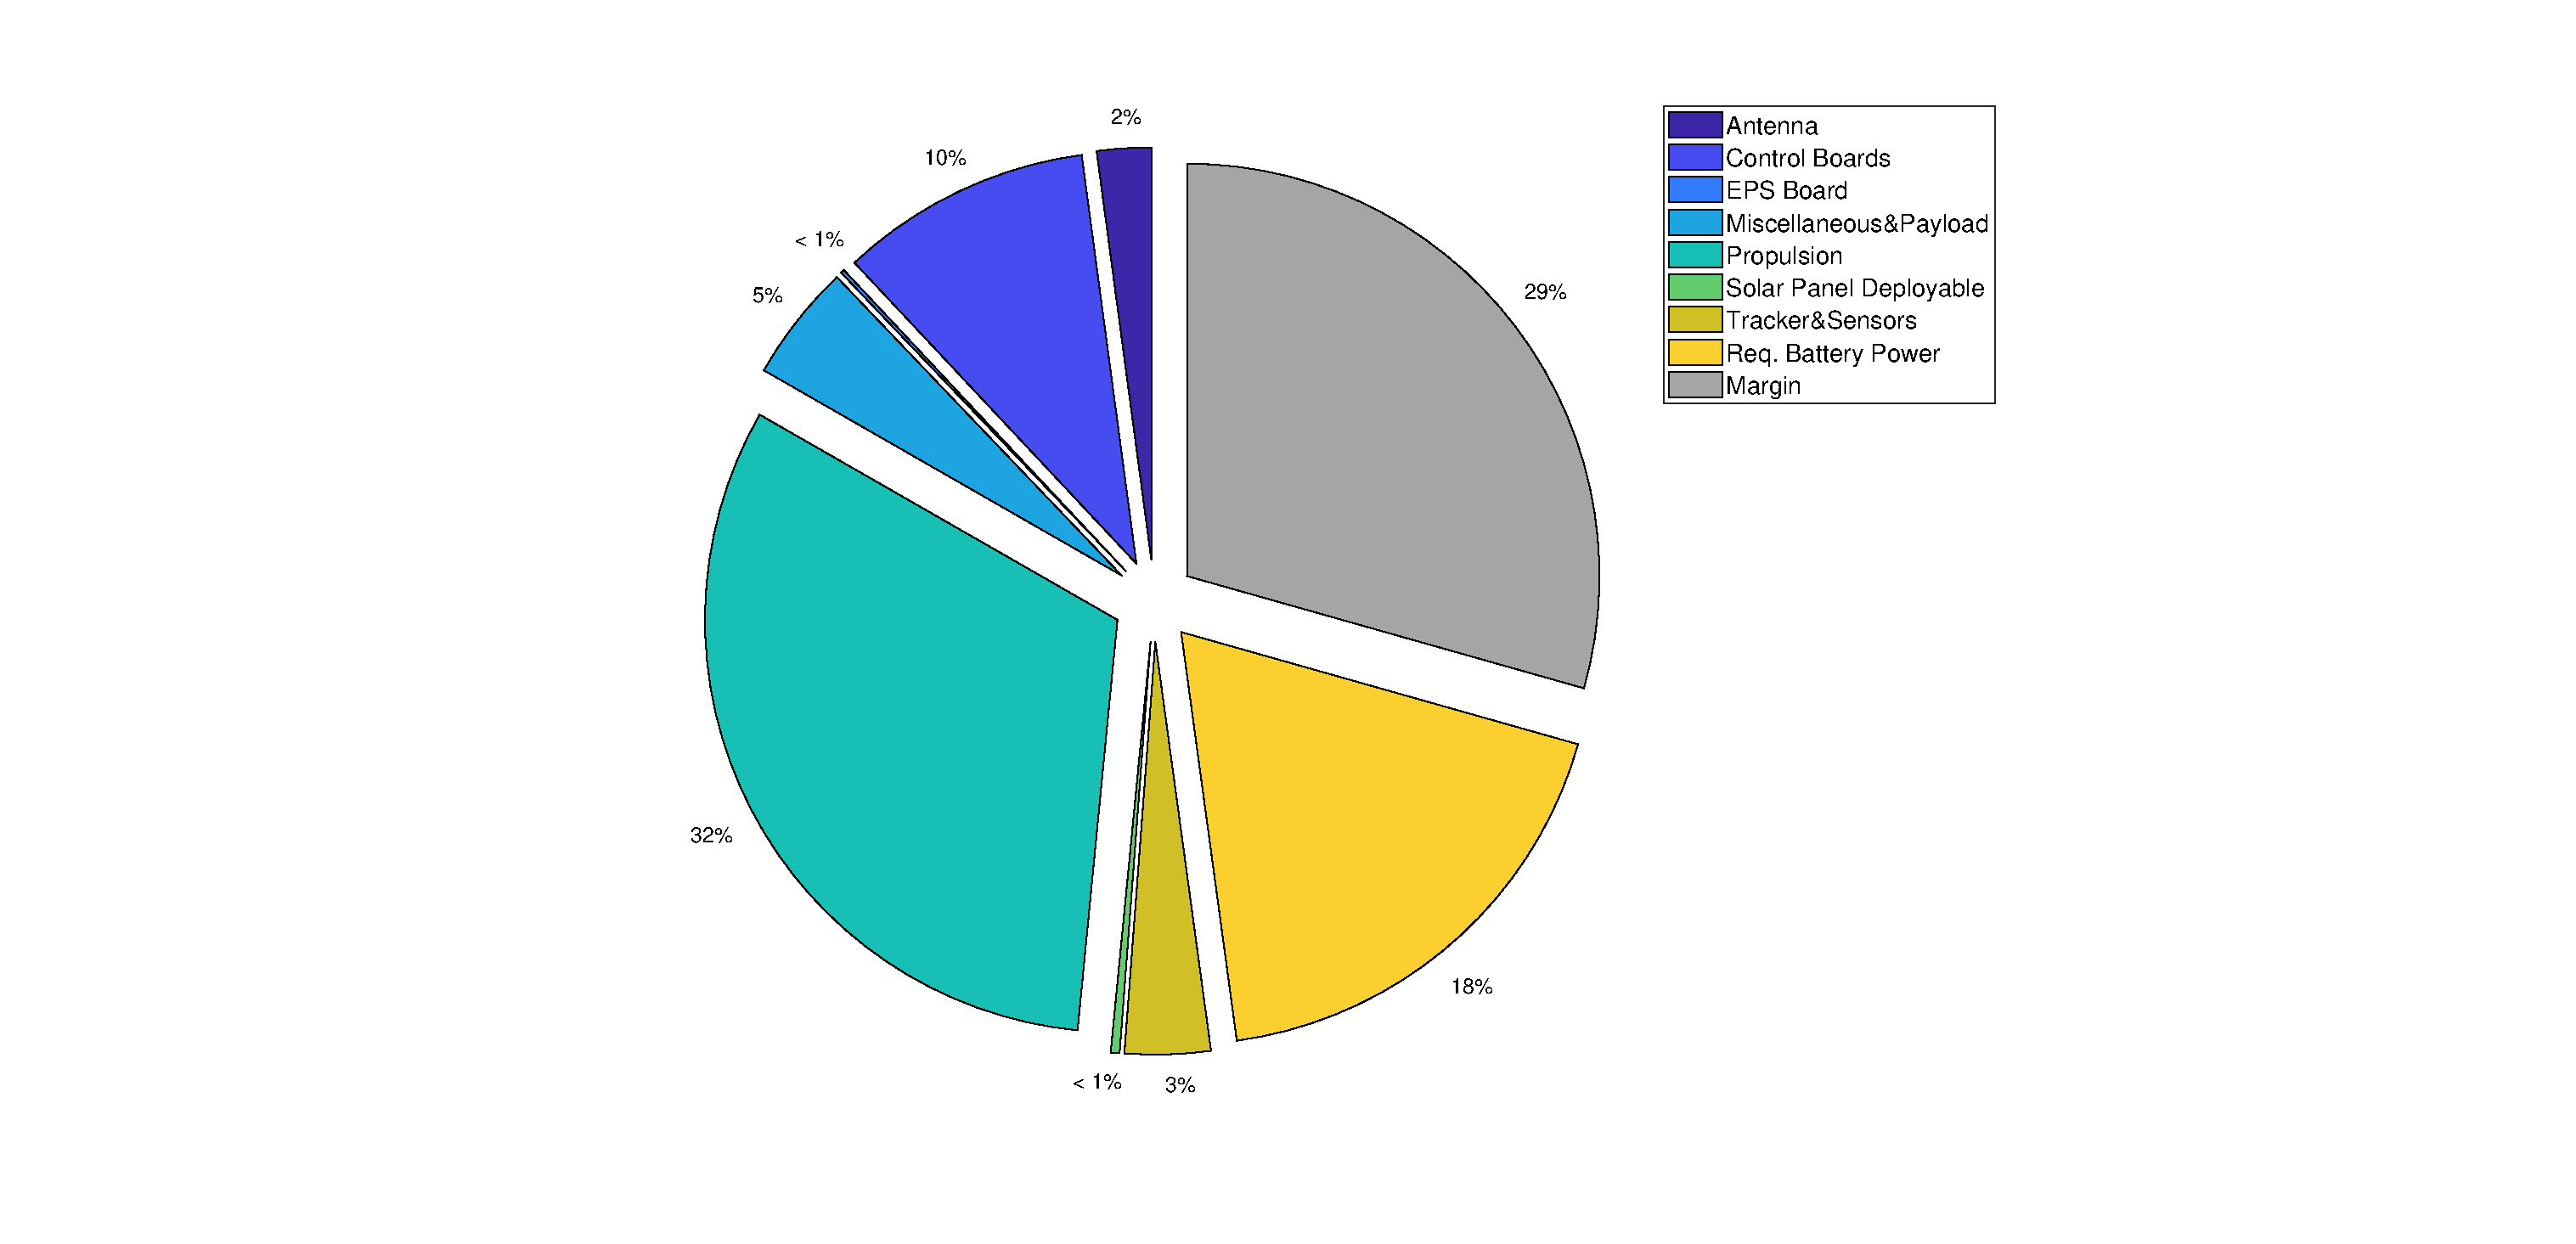
\includegraphics[width=1.50\textwidth]{./Budget/power}
											%\caption{Energiebudget für das angenommene Design}
											%\label{fig:power}
										%\end{figure}
										
										\begin{figure}[H]
											\centering
												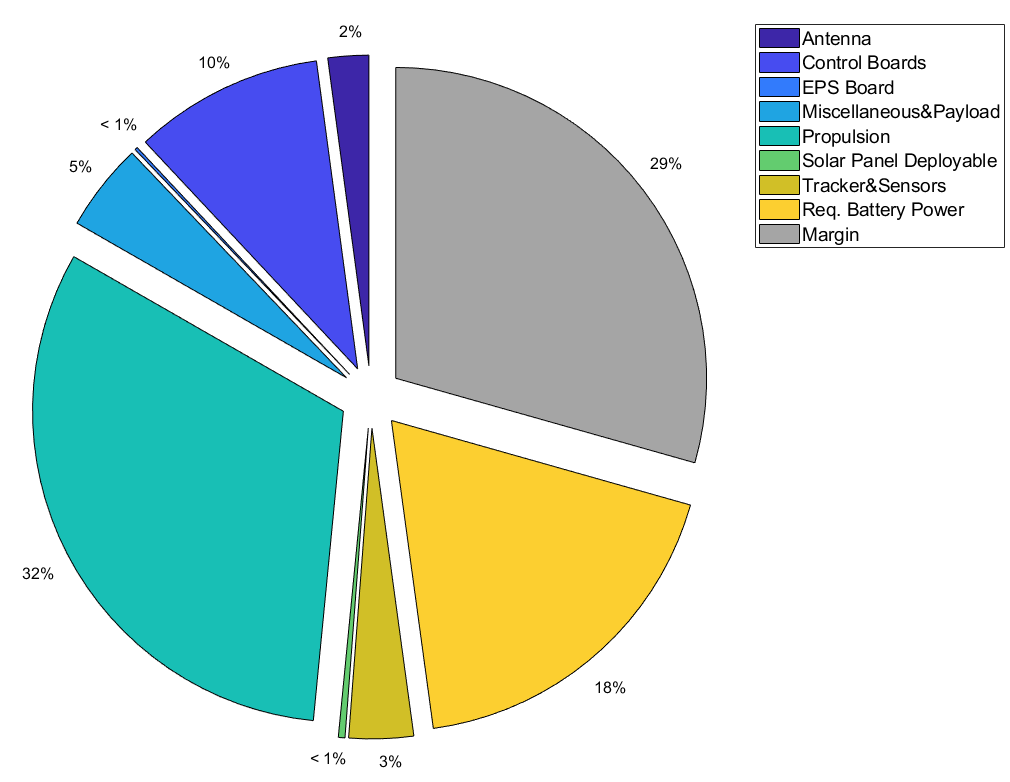
\includegraphics[width=0.90\textwidth]{./Budget/power_neu}
											\caption{Energiebudget für das angenommene Design}
											\label{fig:power}
										\end{figure}
Um das Leistungsbudget zu erstellen, muss die Höhe der Umlaufbahn und der Brennwinkel $\beta$ angegeben werden (\abb{fig:power}). Diese wurden mit \SI{1150}{\kilo\metre} und \num{0}° angenommen (\tab{tab:cubesatdesign}).  Das Programm ermittelt für diese Parameter direkt die Zeit einer Orbitperiode und die dazugehörige Licht- und Schattenzeit. Mit den angenommenen Parametern ergibt sich eine Umlaufdauer von \num{108,34} Minuten bei einer Sonnenzeit von \num{73,48} Minuten. Die im Designe enthaltenen Solarpanele müssen einer Position am CubeSat zugeordnet werden.

Nachdem die maximale Missionsdauer angegeben wurde kann die Energieerzeugung während einer Erdumrundung berechnet werden (\abb{fig:power3} und \abb{fig:power4}). Dabei wird mit einer  Verschlechterung der Energieerzeugung von \num{3}\% pro Missionsjahr gerechnet. Diese spiegelt sich dann in der angepassten Leistung der Solarpanele wieder. Das Programm bezieht außerdem die verschiedenen Beleuchtungsfälle der Solarzellen bei verschiedenen Sonnenwinkeln $\alpha$ ein. Um eine Gesamtenergie berechnen zu können,  werden Wahrscheinlichkeiten für die verschiedenen Beleuchtungsfälle angenommen. Die endgültige Leistung der Konfiguration beläuft sich auf \SI{143,144}{\watt}. Bei einer Sonnenzeit von \num{73,48} Minuten ergeben sich \SI{175,27}{\watt\hour} pro Erdumrundung. 
			
			\begin{figure}[H]
				\centering
					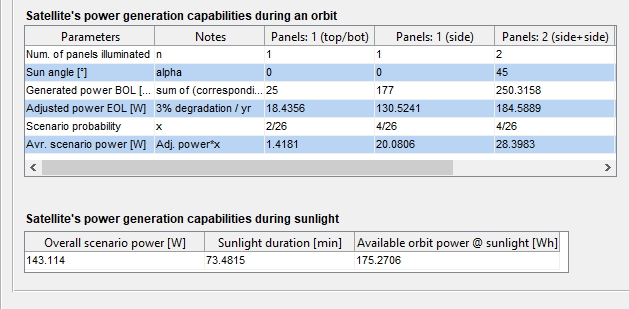
\includegraphics[width=0.70\textwidth]{graphics/power3.png}
				\caption{QuSAD: Energieerzeugung pro Orbit 1}
				\label{fig:power3}
			\end{figure}
			
			\begin{figure}[H]
				\centering
					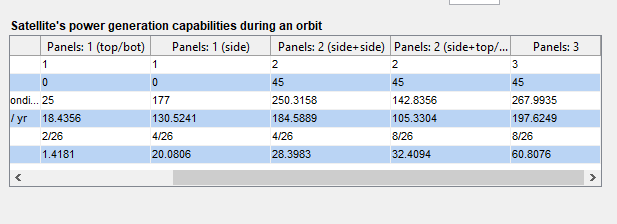
\includegraphics[width=0.70\textwidth]{graphics/power4.PNG}
				\caption{QuSAD: Energieerzeugung pro Orbit 2}
				\label{fig:power4}
			\end{figure}
Da das Haupttriebwerk und das RCS-System nicht dauerhaft betrieben werden, muss für diese Komponenten eine prozentuale Brenndauer angegeben werden. Die mit den getroffenen Annahmen über die Brenndauer veränderten Werte  (\tab{tab:cubesatdesign}) können manuell in QuSAD geändert werden. Für das Haupttriebwerk wurden \num{16,1}\% und das RCS-System \num{0,001}\% Nutzungszeit angenommen. Bei den anderen Komponenten wird von einem dauerhaften Betrieb ausgegangen. Der Energieverbrauch jeder Komponente pro Orbit wird direkt angezeigt. (\abb{fig:power5})
			
			\begin{figure}[H]
				\centering
					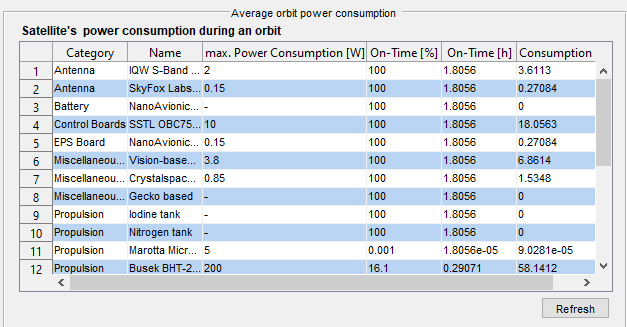
\includegraphics[width=0.70\textwidth]{graphics/power5.png}
				\caption{QuSAD: Energieverbrauch pro Orbit}
				\label{fig:power5}
			\end{figure}
Die von QuSAD angenommenen Werte zur Bestimmung des Energieüberschusses sind in  \abb{fig:power6} zusammengefasst. Es kann genau bestimmt werden wie viel Energie die Konfiguration während der Sonnen- und Schattenperiode zur Verfügung hat und wie viel davon verbraucht wird. Aus dem Budget ist dann der Anteilige Verbrauch der 
einzelnen Komponenten ersichtlich.

			
			\begin{figure}[H]
				\centering
					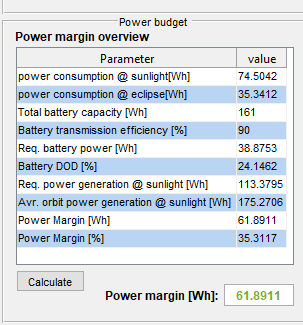
\includegraphics[width=0.45\textwidth]{graphics/power6.png}
				\caption{QuSAD: Überblick Energieüberschuss}
				\label{fig:power6}
			\end{figure}
Zur Berechnung des Budgets wird eine Batterieeffizienz von \num{90}\% angenommen. Der Wert “Power margin” gibt den Energieüberschuss eines Orbits in Wh an (\abb{fig:power6}). Das Budget in \abb{fig:power} stellt den Zustand des CubeSats nach der angegebenen Missionsdauer dar. Die Energieproduktion pro Orbit sinkt mit dem Fortlaufen der  Mission. Somit ist der Energieüberschuss bei Missionsstart deutlich höher. 			
			
			
			
			\section{Auswertung und Optimierung des Designs}
			\hfill\emph{(Florian Czorny, Valentina Dietrich)}
			
Die Auswertung der Ergebnisse zeigt, dass bei der Masse der Konfiguration eine Steigerung von \SI{21,5}{\kilogram} (\num{43}\%) und bei dem Volumen hingegen lediglich eine Steigerung von \SI{815}{\centi\metre\cubed} (\num{3}\%) gemäß QuSAD zulässig ist. Hier lässt sich feststellen, dass das Programm von dem Gesamtvolumen \SI{27000}{\centi\metre\cubed} ausgeht, wobei das maximal verfügbare Volumen bei einem \SI{34 x 35 x 36}{\centi\metre} großen Satelliten mit \SI{42840}{\centi\metre\cubed} festgelegt ist \cite{Lettau.}. Dies weist eine Differenz von \num{36}\% auf. Demzufolge muss bei der Konfiguration ein verfügbares Volumen von \num{39}\% vorhanden sein. Rückwirkend lässt sich feststellen, dass beim Einpflegen der Daten ein zulässiges Gesamtvolumen manuell eingetragen werden muss, andernfalls orientiert sich das Programm an der Dimension, die in diesem Fall mit \SI{27}{\unit} ein Volumen von \SI{27000}{\centi\metre\cubed} aufweist. An dieser Stelle muss beachtet werden, dass bei vielen Komponenten keine genauen Angaben bezüglich der Masse und des Volumens gegeben waren und dementsprechend durch Vergleich mit näherungsweise ähnlichen Systemen oder Aufwärtsskalierung die Werte bestimmt wurden. Zusätzlich kommt bei dem Massenbudget hinzu, dass die Software keine Einbauvorrichtungen berücksichtigt. Demnach würde sich die verfügbare Spanne für Masse als auch Volumen senken. Bei dem Leistungsbudget muss beachtet werden, dass der erhöhte Verbrauch während des RDVDO nicht berücksichtigt wird. An dieser Stellen empfiehlt sich eine weitere Untersuchung. Den Ergebnissen zufolge lässt sich die betrachtete Mission mit dem aktuellen Stand des Designs durchführen und demzufolge ist bislang keine Optimierung erforderlich. Da in dem aktuellen Entwurf viele Unsicherheiten vorhanden sind und einige Aspekte durch das Leistungsbudget nicht beachtet worden sind, wie die Tankmasse, könnte eine Optimierung nach der Missionsanalyse notwendig sein. 
														% -"- CubeSat Design 														
	\chapter{Missionsdesign und Simulation}

%\section{Bewertungsstrategie}
	%Die Strategie besteht draus mehrere Simulationen per GMAT für untershciedliche Koonfigs durchzuführen. Die Bewertung fokusiertsich auf die Machbarkeit des De-orbiting (seihe TODOS.txt)\\
	%	\subsection{Kriterien der Bewertung}
%-------------------------------------------------------------Missionsbeschreibung

\section{Missionsbeschreibung}
\hfill\emph{(Frederik Schäfer)}\\	
	Ziel der Mission ist es defekte, nicht kooperative Satelliten von Megakonstellationen (z.B.: Starlink) abzubremsen, sodass sie in der Erdatmosphäre verglühen und das Kollisionsrisiko minimiert wird. Das Höhen- und Gewichtsintervall wurden auf \num{400}-\SI{1400}{\kilo\metre}, bzw. \num{50}-\SI{5000}{\kilogram} festgelegt, da alle Satelliten bisher geplanter Megakonstellationen innerhalb dieser Intervalle befinden.
Es wird angenommen, dass sich der CubeSat und das Ziel zu Beginn in derselben Umlaufbahn befinden und nur wenige Kilometer voneinander entfernt sind. Das Haupttriebwerk wird für RDV und Docking nicht verwendet, sodass für den Wiedereintrittsvorgang die gesamte Kraftstoffmenge zur Verfügung steht. Sobald beide Satelliten miteinander Verbunden sind richten sie sich so aus, dass das Haupttriebwerk des CubeSats entgegen der Bewegungsrichtung wirkt. Als nächstes beginnt der eigentliche Deorbit Vorgang. Hier fängt auch die jeweilige Simulation an. Da die Solarzellen den Antrieb nicht dauerhaft versorgen können, wird ein Brennwinkel von \num{58}° um die wahre Anomalie (Apogäum) festgelegt. Jeder Brennvorgang verringert die Geschwindigkeit und senkt somit das Perigäum ab. Die Mission ist erfolgreich, wenn das Perigäum eine Höhe von \SI{180}{\kilo\metre} erreicht hat. Die Simulation wird nach zehn Jahren abgebrochen, wenn die Mission bis dahin nicht erfolgreich war. 
Zuerst wird eine \textbf{erste Mission} simuliert, die eine kreisförmige Umlaufbahn annimmt und das Höhenintervall in \SI{50}{\kilo\metre} Schritten erhöht. Die Masse wird von \num{50} bis \SI{550}{\kilogram} in \SI{25}{\kilogram} und von \num{600} bis \SI{5000}{\kilogram} in \SI{100}{\kilogram} Schritten erhöht.
Mit der \textbf{zweiten Mission} wird betrachtet, wie sich die Deorbitzeit für ausgewählte Massen verhält, wenn die Exzentrizität verändert wird. Das Höhenintervall beschreibt hierbei die Höhe des Perigäums und die Exzentrizität wird von \num{0.025} bis \num{0.3} betrachtet.
	
			
%-------------------------------------------------------------GMAT
\section{GMAT}
		\subsection{Beschreibung der Software}
		
		Der GMAT Mission Planner ist ein Open Source Programm, welches von der NASA entwickelt wird \cite{Hughes.}. Das Programm ist dazu da um Trajektorien von Satelliten zu berechnen und optimieren. Der Missionsraum umfasst das gesamte Sonnensystem und erlaubt es die Gravitationseinflüsse von allen größeren Himmelskörpern in die Berechnungen mit einfließen zu lassen. 
Die Eingabe der gewünschten Parameter erfolgt über ein GUI oder ein benutzerdefiniertes Skript. Die Skriptsprache von GMAT lehnt an der von MathWorks MATLAB\textregistered \space an.
Das GUI beinhalted einen 3D Plot und einen 2D Plot. Der 3D Plot zeigt die Position und Trajektorie des Satellitens im dreidimensionalen Raum während der 2D Plot eine Projektion der Trajektorie auf die Oberfläche eines gewählten Himmelskörpers zeigt.

\begin{figure}[!h]
	\centering
		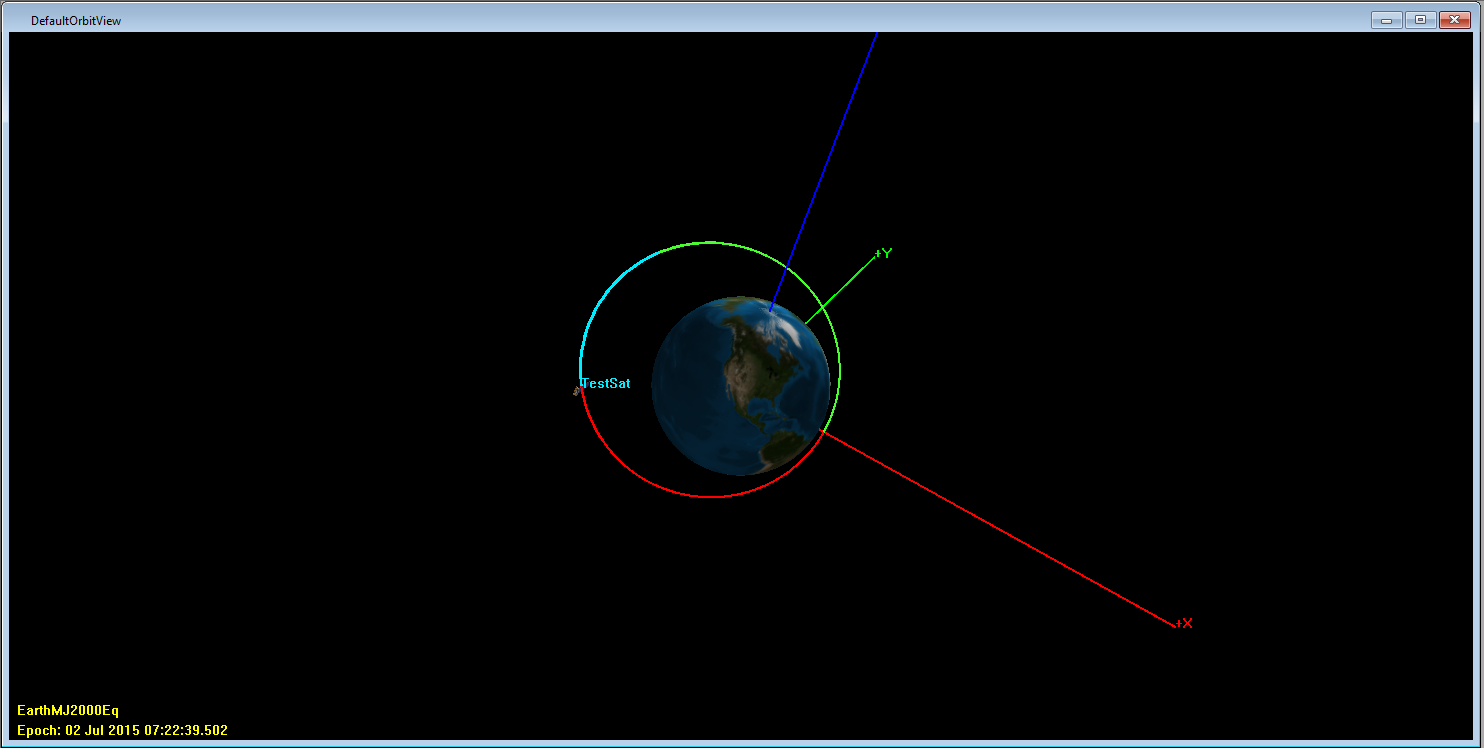
\includegraphics[width=1.00\textwidth]{graphics/GMAT/GMAT_OrbitView2.PNG}
		\caption{3D Plot eines Satelliten in einer exzentrischen Umlaufbahn um die Erde}
			\label{fig:OrbitView2}
\end{figure}


	Im GUI finden sich drei Reiter: ’Resources’, ’Mission’ und ’Output’.\\
In dem Resources Reiter werden alle Ressourcen die für die Mission benötigt werden eingestellt. Dazu gehören die Schubdüsen, Tanks, Startumlaufbahn des Satelliten und andere Dinge, die während der Mission im Hintergrund wichtig sind.\\
Im Missions Reiter werden nacheinander die auszuführenden Befehle aufgelistet. Diese können auch mit Logikoperatoren wie While- oder Forschleifen wiederholt werden.\\
Im Output Reiter finden sich nach dem Missionsdurchlauf die Ausgaben die im Laufe der Mission erfasst worden sind wieder. 


%-------------------------------------------------------------Kreisorbitskript

\subsection{Missionsskript 1}


Im Folgenden ist das Skript für die erste Simulation beschrieben. Die Wahl viel auf eine Whileschleife, da Forschleifen in GMAT nicht abbrechen, wenn der Wert innerhalb der Schleife verändert wird.
Das ist für dieses Skript jedoch benötigt, da die beiden letzten if-Abfragen dafür sorgen, dass die benötigte Simulationszeit minimiert wird.
Die erste if-Abfrage ist notwendig, da bei einigen Simulationen die Treibstoffmasse ins negative ging.
Die zweite und dritte if-Abfrage könnten in einer if - else if -Abfrage kombiniert werden, aber diese Logik ist in GMAT nicht enthalten.
Alle if-Abfragen, die den Abbruchwert verändern sind dazu da ermitteln zu können warum die innere Whileschleife beendet worden ist. \\ 

\begin{algorithmic}

\STATE Setze die aktuelle Kreisbahnhöhe auf die erwünschte Starthöhe
\WHILE{Aktuelle Kreisbahnhöhe <= Gewählte Endhöhe}
\STATE Setze aktuelle Zielmasse auf die erwünschte Startmasse
\WHILE{Aktuelle Zielmasse <= Gewählte Endmasse}
\STATE Setze Abbruch auf 0
\STATE Setze Start Orbitparameter zurück
\STATE Setze Tankmasse zurück
\RETURN Report bei Start neuer Höhen- und Massekombination

\WHILE{Abbruch == 0}

\IF{Treibstoffmasse > 0.001} 
\STATE Fortbewegen zu einer wahren Anomalie von 151°
\STATE Triebwerk einschalten
\STATE Fortbewegen bis zu einer wahren Anomalie von 209° oder Treibstoffmasse von 0.00095 
\STATE Triebwerk ausschalten
\ENDIF

\IF{Aktuelle Höhe des Perigäums > 6558}
\STATE Fortbewegen zum Perigäum
\ENDIF

\IF{Aktuelle Höhe des Perigäums <= 6558}
\STATE Setze Abbruch auf 1
\ENDIF

\IF{Aktuelle Exzentrizität < 0.0025}
\STATE Setze Abbruch auf 2
\ENDIF

\IF{Vergangene Zeit in Tage >= 3700}
\STATE Setze Abbruch auf 3
\ENDIF

\RETURN Report am Ende von jedem Durchlauf der Whileschleife
\ENDWHILE

\RETURN Report nach Abschluss jeder Whileschleife

\IF{Abbruch == 3}

\IF{Aktuelle Zielmasse == gewählte Startmasse}
\STATE Setze aktuelle Kreisbahnhöhe auf Wert größer als Endhöhe 
\ENDIF

\STATE Setze aktuelle Zielmasse auf Wert größer als Endmasse
\ENDIF

\STATE Inkrementiere Masse um gewählten Wert
\ENDWHILE

\STATE Inkrementiere Höhe um gewählten Wert
\ENDWHILE

\end{algorithmic}

\\
\begin{center}
\begin{tabular}{c| c{5cm}}
\label{Abbruchkrit}
Abbruchwert & Erklärung \\
\hline \hline
1 &  \multicolumn{2}{p{12cm}}{ Bricht die Whileschleife ab, wenn das Perigäum unter \SI{180}{\km} ist. Die Mission ist erfolgreich verlaufen}\\ \hline
2 &  \multicolumn{2}{p{12cm}}{ Bricht die Whileschleife ab, wenn die Exzentrizität unter 0.0025 ist. Wird die Exzentrizität zu gering, gibt GMAT einen Fehler aus}\\  \hline
3 &  \multicolumn{2}{p{12cm}}{ Bricht die Whileschleife ab, wenn die vergangene Zeit 3700 Tage überschreitet. Die Mission ist nicht erfolgreich verlaufen}\\  
\end{tabular}
\end{center}



%	Bevor die Mission in die Schleifen geht wird die Starthöhe über $Initial Orbitheight$ festgelegt. Danach geht es in die $Orbit Height$-Schleife und die Startmasse wird festgelegt.
%Die nächste Schleife durchläuft alle Massen. Die Endwerte für beide Schleifen werden in $End\_mass$ und $End\_height$ festgelegt. Das Inkrement erfolgt am Ende jeder Schleife in $Inkrement mass$ bzw $Inkrement height$.\\
%Im Kern diesen Skriptes steht die Whileschleife.\\
%Nach einer Überprüfung des Treibstoffstands wird der Satellit mit dem ersten Propagator Befehl bis auf eine wahre Anomalie von 151° vorangebracht. 
%Danach wird der Schubbefehl gestartet und der Propagator $PropToBurnEnd$ lässt den Satelliten, während dieser Schub gibt, bis zu einer wahren Anomalie von 209° vorlaufen. Sollte der Treibstoff zuvor auf 0 fallen wird dieser Vorgang abgebrochen. Danach wird der Schub beendet.

%Aufgrund einiger Fehler, die während des Testens dieses Skripts aufgetreten sind, folgen jetzt einige If-Abfragen, die als Abbruchbedingungen der Kernschleife dienen.
%Die erste überprüft ob das Perigäum des Satelliten größer als 6558 ist. Ist dies der Fall wird der Fortlauf bis zum Perigäum durchgeführt. Die Zweite If-Abfrage überprüft das Gegenteil, also ob das Perigäum kleiner oder gleich 6558 ist. Ist dies der Fall wird die Variable “Abbruch” auf 1 gesetzt. Der Grund für diese beiden If-Abfragen liegt darin, dass die Whileschleife bei einigen Simulationen nicht auf einen zu niedrige Wert reagiert hat. Außerdem kam es vor, dass die Simulation immer langsamer wurde, wenn der Satellit bei einer kleinen Großen Halbachse zum Perigäum navigiert ist. Das wurde dadurch umgangen, dass nur zum Perigäum navigiert wird, wenn diese über 6558 ist. \\
%Die nächste If-Abfrage überprüft ob die Exzentrizität niedriger als 0.0025 ist. Ist dies der Fall wird der Wert “Abbruch” auf 2 gesetzt. Mit dieser If-Abfrage wird ein Fehler umgangen, der bei den niedrigen Zielhöhen häufiger aufgetreten ist. Ab einem gewissen Punkt in der Simulation von geringen Höhen verringert sich die Exzentrizität wieder, da durch atmosphärischen Drag das Apogäum schneller sinkt als Das Perigäum durch den Schub. Dies hatte aus unerfindlichen Gründen einen Error zur Folge, zu dem kein fix gefunden wurde. \\
%Die letzte Abbruchbedingung ist die 10 Jahresmarke. Hier wird abgefragt, ob die Tage seit dem Start der Whileschleife größer als 3700 Tage sind. Ist dies der Fall wird die Variable Abbruch auf 3 gesetzt.\\
%Der letzte Befehl in der Kernschleife ist der EndWhile Report. Hier wird dem Programm gesagt, dass er die gewünschten Daten in eine Datei speichern soll. Diese Datei dient lediglich dazu ungeklärte Abbrüche und Abstürze zu ermitteln und war für die Auswertung irrelevant.\\
%Die Whileschleife läuft solange, bis das Abbruchkriterium $\neq 0$ ist.\\
%Danach werden noch zwei Reports angefertigt, wobei der AWReport in eine separate Datei, die zur Auswertung genutzt wurde, schreibt.\\
%Nach der Kernschleife wird überprüft ob das Abbruchkriterium 3 war. Ist dies der Fall bedeutet das, dass die Nachfolgenden Masseschritte auch nicht in unter 3700 Tagen geschafft werden können. An dieser Stelle wird die Aktuelle Masse auf einen Wert der höher ist als die gewählte Endmasse und die Masseschleife wird abgebrochen um Zeit zu sparen. Die letzte If-Abfrage ist eine weitere Maßnahme um Zeit zu sparen. Hier wird abgefragt, ob die Aktuelle Masse gleich der gewählten Startmasse ist. Ist dies der Fall wird die äußerste Whileschleife beendet und die Mission ist fertig simuliert.\\
%Vor der Kernschleife stehen noch einige Equation Befehle, welche unter Anderem den Orbit und das Datum zurücksetzen. Außerdem wird der “Abbruch”-Wert auf 0 zurückgesetzt.




%-------------------------------------------------------------Exzen.Skript

\subsection{Missionsskript 2}

	Für die zweite Untersuchung wurde das Skript so modifiziert, dass es die Exzentrizitäten von \num{0.025} bis \num{0.3} durchläuft.
Der Aufbau der Kernschleife ist gleich geblieben. Die erste Schleife um die Kernschleife ist eine Forschleife,, die die Exzentrizität in \num{0.025}er Schritten Inkrementiert. Innerhalb dieser Schleife wird zu Beginn das Perigäum auf die Starthöhe gesetzt und das Apogäum mit der Exzentrizität über
\begin{equation}
r_A = \frac{1+e}{1-e}\cdot r_P
\label{apoapsis}
\end{equation}
berechnet.\\

	In diesem Skript erfolgt die Einstellung der Targetmasse manuell, da nur drei Massen, in unregelmäßigen Abständen, berechnet worden sind. Die äußerste Forschleife ist für die Höhe zuständig und läuft mit einem Inkrement von \SI{100}{\kilo\metre} von \num{400} bis \SI{1400}{\kilo\metre} durch. 
\begin{figure}[!h]
	\centering
		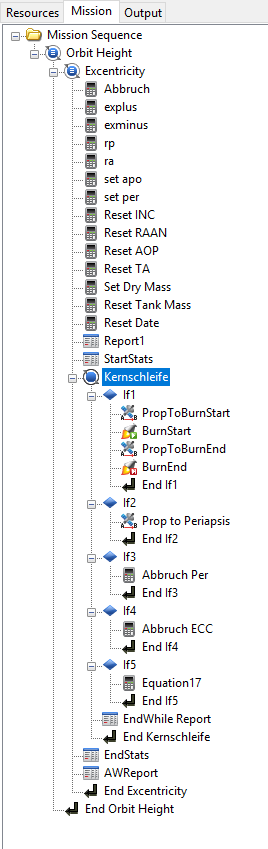
\includegraphics[width=0.35\textwidth]{graphics/GMAT/GMAT_Skript_ECC.PNG}
		\caption{Deorbitskript - Variation der Exzentrizität}
			\label{fig:GMAT_Skript_ECC}
\end{figure}



%-------------------------------------------------------------Ergebnisse


\section{Ergebnisse}

	Im Folgenden werden die Ergebnisse der zwei durchgeführten Simulationsarten präsentiert.
\begin{figure}[h]
\centering
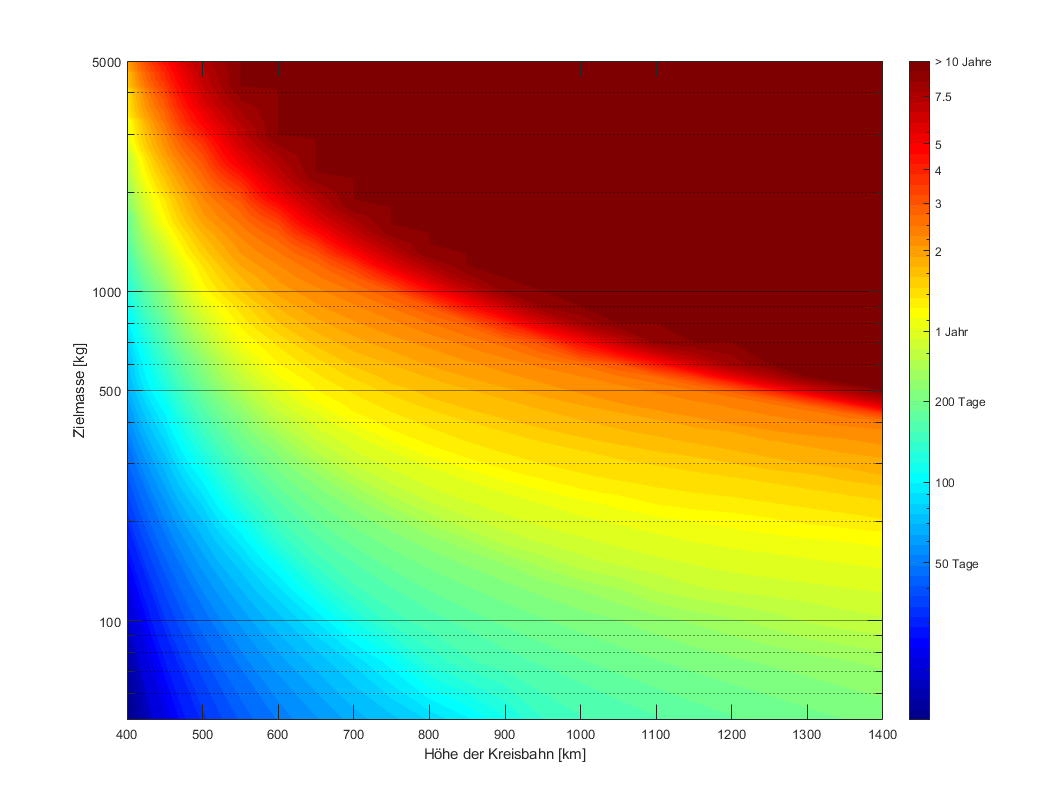
\includegraphics[width=1.00\textwidth]{./graphics/GMAT/GMAT_Mass_over_Height.png}
\caption{Simulationsergebnisse 50-5000kg, Kreisorbit}
\label{fig:GMAT_Mass_over_Height}
\end{figure}

\subsection{Mission 1}

	In Abb. \ref{fig:GMAT_Mass_over_Height} sind die zugehörigen Wiedereintrittszeiten farblich in Abhängigkeit von Masse und Starthöhe abgetragen. Die Zeitskala ist logarithmisch von \num{0} bis \num{10} Jahre an der Seite aufgeführt.  
Es ist klar zu erkennen, dass niedrigere die Massen auch aus vergleichsweise großen Höhen entfernt werden können. Die maximale Höhe des Zielsatelliten nimmt jedoch mit zunehmender Masse stark ab, wenn die Zeitvorgabe von maximal \num{10} Jahren eingehalten werden soll.

	Eine detaillierte Ansicht der Massen von \num{50} bis \SI{550}{\kilogram} bietet \abb{fig:GMAT_Mass_over_Height_550}, da diese mit einer viermal höheren Auflösung (\SI{25}{\kilogram} Schritte) simuliert worden ist. Hier wird es deutlicher, dass die Zielmasse bei \SI{1400}{\kilo\metre} maximal \SI{500}{\kilogram} betragen darf, um das Limit von zehn Jahren nicht zu überschreiten.

\begin{figure}[h!]
	\centering
		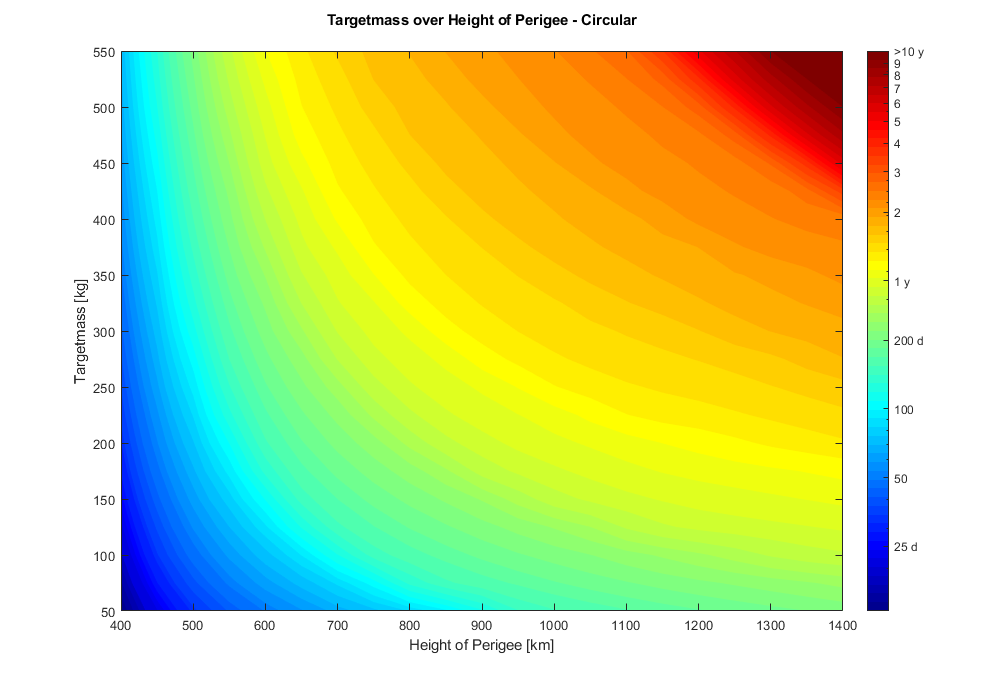
\includegraphics[width=1.00\textwidth]{./graphics/GMAT/GMAT_Mass_over_Height_550.png}
		\caption{Simulationsergebnisse 50-550kg, Kreisorbit}
	\label{fig:GMAT_Mass_over_Height_550}
\end{figure}


	Durch die logarithmische Skala der Zeit ist klar erkennbar wie sehr die benötigte Zeit für die Mission ansteigt, nach dem der Treibstoff nach ca. \num{3} Jahren (hellroter Bereich) aufgebraucht worden ist. Unterhalb dieses Bereichs nimmt die Missionsdauer nur langsam zu, wenn Umlaufbahn oder Masse erhöht werden. Oberhalb ist ein deutlich schnellerer Übergang zum dunkelroten Bereich erkennbar, der eine Missionsdauer von über \num{10} Jahren bedeutet. Dies geschieht im Bereich um drei Jahre. Je höher die Starthöhe, desto länger brennt das Triebwerk pro Umlauf, da die \num{58}° Brennwinkel mehr Zeit benötigen um durchlaufen zu werden. 

\subsubsection{Ergebnis Mission 1}

	Die gewählte Konfigurationen kann Satelliten mit einem Gewicht von \SI{375}{\kilogram} (Starlink) und einer Erdumlaufbahn von \SI{1400}{\kilo\metre} innerhalb von \num{2} Jahren  aktiv zum Wiedereintritt verhelfen. Für niedrigere Höhen wird dieser Vorgang schon früher abgeschlossen. 

	Bei großen Höhen ist die maximale Masse limitiert, jedoch ist der Aerodynamische Widerstand in geringen Höhen so stark, dass Trümmerteile bis zu zwei Tonnen innerhalb eines Jahres aus ihrer Umlaufbahn entfernt werden können. 

\subsection{Mission 2}

	Die Abbildungen \ref{fig:GMAT_ecc_a}, \ref{fig:GMAT_ecc_b} und \ref{fig:GMAT_ecc_c} repräsentieren die Ergebnisse für die ausgewählten Massen \num{50}, \num{375} und \num{550}\si{\kilogram}. Die benötigte Missionszeit wird hier in Abhängigkeit von Exzentrizität und Starthöhe des Perigäums dargestellt. Die Zeitskala ist wieder logarithmisch von \num{0} bis \num{10} Jahre an der Seite aufgeführt.


\begin{figure}[h]
	\centering
		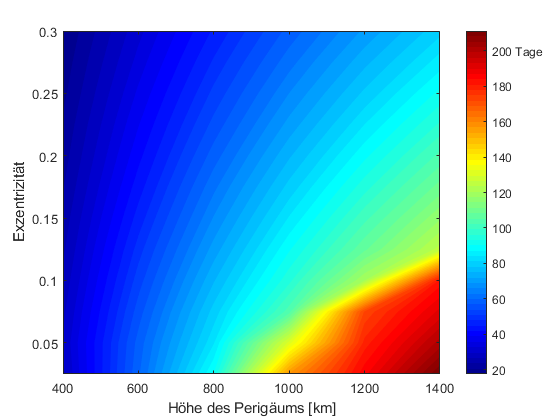
\includegraphics[width=0.80\textwidth]{./graphics/GMAT/ecc_perigee_50kg.png}
		\caption{Simulationsergebnisse Variation der Exzentrizität, 50 kg}
	\label{fig:GMAT_ecc_a}
\end{figure}

	Auffallend ist die Tatsache, dass eine höhere Exzentrizität eine geringere Missionszeit zur Folge hat. Der Grund hierfür ist unter Anderem, dass bei hohen Exzentrizitäten der CubeSat länger innerhalb der \num{58}° um das Apogäum ist und das Triebwerk somit länger brennt. Im Fall von \SI{550}{\kilogram} zeigt \abb{fig:GMAT_ecc_c}, dass obwohl es über alle Höhenstufen zu einer Verkürzung der Mission kommt, dies für \SI{1400}{\kilo\metre} trotzdem über \num{10} Jahre dauert. 
	
	\begin{figure}[h]
	\centering
		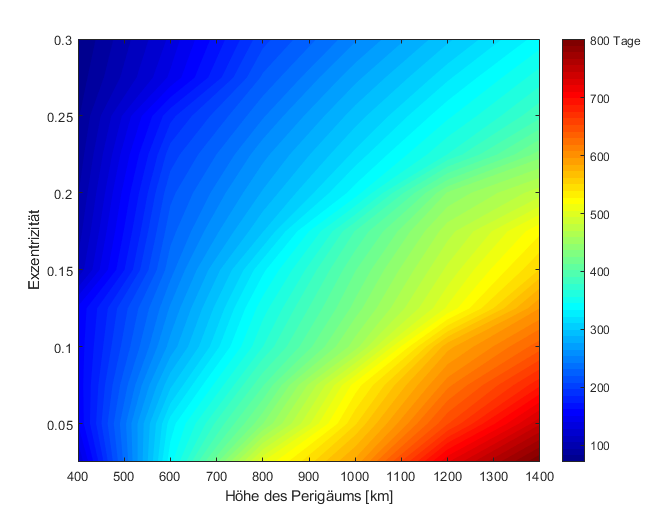
\includegraphics[width=0.80\textwidth]{./graphics/GMAT/ecc_perigee_375kg.png}
		\caption{Simulationsergebnisse Variation der Exzentrizität, 375 kg}
	\label{fig:GMAT_ecc_b}
\end{figure}

\subsubsection{Ergebnis Mission 2}
Das Ergebnis der zweiten Missionssimulation ist, dass die Exzentrizität keinen negativen Einfluss auf die Wiedereintrittzeit hat. Wurde über die erste Simulation festgestellt, dass die Mission erfolgreich war, so ist davon auszugehen, dass eine Mission mit der selben Starthöhe (Kreisbahnhöhe = Perigäumshöhe) auch erfolgreich ist.

\begin{figure}[h]
	\centering
		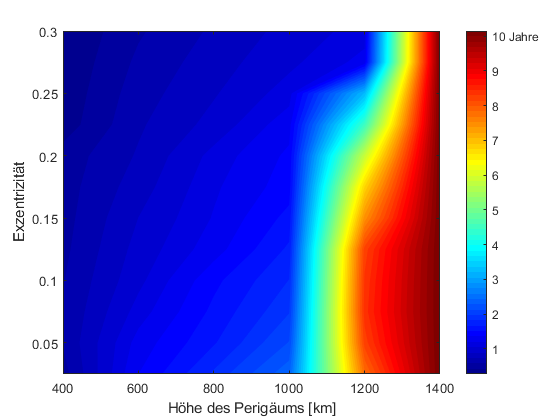
\includegraphics[width=0.80\textwidth]{./graphics/GMAT/ecc_perigee_550kg.png}
		\caption{Simulationsergebnisse Variation der Exzentrizität, 550 kg}
	\label{fig:GMAT_ecc_c}
\end{figure}


%For every considered satellite design (=mainly thruster configuration, 3-4 different designs), generate following data: \\
%
%Deorbit time and spent fuel mass for all:
%\begin{itemize}
	%\item Masses from 50-500 kg\\
	%\item Altitudes from 1400-400? km  (ggf. semi-major axis) \\
	%\item Eccentricities from ~0 to highest recorded eccentricity of debris in <1400 km orbit
%\end{itemize}
%
%Note: Output EVERY relevant simulation parameter (initial orbit and S/C data, burn start/stop angles, start epoch etc.)  at the beginning of every simulation run [discuss with Max]
	%
			%\subsection{Reachability Enveloppe}
%RESULTING DIAGRAMS: \\
%
%\begin{enumerate}
		%\item Visualize the absolute performance of the main design (Max), e = 0 \\
				%\begin{itemize}
						%\item Axes: y = mass, x = SMA \\
						%\item Graph: Use color gradients to display deorbit times (same time = same color)
				%\end{itemize}
				%\item  Visualize the influence of eccentricity on deorbit times using the main design \\
				%\begin{itemize}
						%\item Axes: y = mass, x = SMA \\
						%\item Select a fixed deorbit time (e.g. 2 years) \\
						%\item Graph: Use color gradients to display eccentricities (same ecc = same color)
				%\end{itemize}
				%\item Visually compare the performances of the different designs (Max \& 2-3 group designs), e = 0 
				%\begin{itemize}
						%\item Axes: y = mass, x = SMA \\
						%\item Select 1-2 fixed deorbit times (e.g. 2 years \& 5 years) \\
						%\item Graph: Draw lines of same deorbit time (selected above) for each of the different designs
				%\end{itemize}				
%\end{enumerate}
%Optional for group after 3. (decide if worth it)\\
%4. Repeat 1. with all other chosen designs\\
%
%NOTES: \\
%
%For 1. \& 4.:\\
%(Deorbit time limited to 10 years (15? 20?)) \\
%-> <2 years of deorbiting takes 3-4 mins to simulate, amount of data is immense => limit maximum deorbit time? \\
%-> At which deorbiting time does a feasible solution become unattractive? If 200 kg in 1000 km orbit is \\
   %deorbitable in 20 years, is it worth it? Better use chemical deorbiting = different mission in this case? \\
%---> Agree on a meaningful limit on deorbit time \\
%
%For all graphs/simulations: \\
%Fuel mass limited by design -> if 27U standard is to be kept no matter which thruster configuration is \\
%chosen, then smaller/more lightweight thrusters would result in more available space for fuel \\
%---> Agree on a set percentage of margin for all designs (e.g. 50\%) and determine maximum fuel from there? \\
%
%-> For Max's design, fuel mass limited to 10 kg (thinking about increasing to 15 kg)\\
			%\subsection{Missionsauslegung}
					%\textbf{Mögliche CubeSat Konfigurationen}\\
			%\subsection{Missionssimulation}
					%\textbf{Impuls-basierter Schub}\\
					%\textbf{Begrenzter Schub}\\
					%\textbf{Mission mit Randbedingungen}\\
			%\subsection{Konfigurationsvergleich}
					%\textbf{..}\\
					%\textbf{..}\\
					%\textbf{..}\\														% -"- Mission Design												
  \chapter{Fazit und Ausblick}
	\hfill\emph{(Florian Czorny, Valentina Dietrich, Oussama Mouhaya, Frederik Schäfer, Marc Strempel)}	\\
Wie die Arbeit gezeigt hat, kann mit Einschränkungen angenommen werden, dass das vorgeschlagene CubeSate Design in der Lage ist Starlink ähnliche Ziele aus Höhen von \num{400} bis \SI{1400}{\km} aktiv wieder eintreten zu lassen. Bei den GMAT-Simulationen wurde angenommen, dass durchgehend die maximale Leistung zu jedem beliebigen Zeitpunkt verfügbar ist. Dabei wurde auch der Schatten der Erde nicht Berücksichtigt. Mit Einbeziehung diese Faktors kann sich die benötigte Zeit verändern. Bei der Budgetierung mit QuSad wurden teilweise nur angenäherte Werte verwendet. Einige Werte für die verwendeten Systeme wurden auf Basis von existierenden Systemen abgeleitet und skaliert. Daraus kann eine Veränderung der Massen und des Volumens erfolgen. Über sämtliche Komponenten bei denen eine Skalierung stattgefunden hat, sollte Rücksprache mit den Herstellern gehalten werden, um möglichst reale Werte für die Berechnungen zur Verfügung zu haben.  Veränderungen der Masse aufgrund des Treibstoffverbrauchs, sowie die Verringerung der Umlaufbahn  wird nicht berücksichtigt. Eine Rückkopplung beider Programme fand statt, indem eine Konfiguration mit beiden Programmen getestet wurde. Zu beachten ist, dass die genannten Vereinfachungen in Kombination für weitere Abweichungen sorgen. Aus diesem Grund sind die Ergebnisse nur als Richtwerte anzusehen und sollten bei Bedarf mit einer weiterführenden Analyse genauer betrachtet werden. Mit Hilfe der Simulationen konnte gezeigt werden, dass mit dem selben Aufbau auch deutlich größere Massen als die der bekannten Megakonstellationssatelliten abgebremst werden können. Selbst bei einer Höhe von \SI{1400}{\km} verlief die Simulation mit \SI{475}{\kilogram} noch erfolgreich. Die derzeit größte bekannte Masse geplanter Megakonstellationssatelliten liegt mit \SI{386}{\kilogram} deutlich unter diesem Wert \cite{BenLarbi.2017}. Bei der simulierten Konfiguration war die Treibstoffmenge (\SI{10}{\kilogram}) der limitierende Faktor. Durch eine Erhöhung der Treibstoffmasse um \num{50}\% könnte die Zielgruppe auf größere Massen in höheren Umlaufbahnen erweitert werden. Dies lässt sich unter Berücksichtigung des tatsächlichen CubeSat-Volumens von \SI{42840}{\cubic\cm} laut der erstellten Budgets realisieren.  Zielsetzung der vorliegenden Arbeit war die Eignung des angenommen CubeSat Designs für ADR Missionen zu testen. Da in den Simulationen die selbst gesetzten Ziele erreicht worden sind, benötigt das gewählte Design keine grundlegende Veränderung. Anhand der Ergebnisse scheint die Durchführbarkeit einer ADR Mission mit CubeSats realisierbar zu sein. Anknüpfend an diese Ergebnisse scheint es sinnvoll den Fokus nun auf das RDVDO in Verbindung mit dem RCS und der Sensorik zu lenken.
	
	%===================================================
  %
  % Literaturverzeichnis
  %
  %---------------------------------------------------
  \addcontentsline{toc}{chapter}{Literaturverzeichnis}
   \bibliographystyle{ieeetr}
		\bibliography{literaturen}

  
  %===================================================
  %
  % Abbildungsverzeichnis
  %
  %---------------------------------------------------
	\addcontentsline{toc}{chapter}{Abbildungsverzeichnis}
  \listoffigures
  \newpage
  
  %===================================================
  %
  % Tabellenverzeichnis
  %
  %---------------------------------------------------
	\addcontentsline{toc}{chapter}{Tabellenverzeichnis}
		\listoftables																										% Tabellenverzeichnis
			\newpage
  
  %===================================================
  %
  % Symbol- und Abkürzungsverzeichnis
  %
  %---------------------------------------------------
 %\chapter*{Symbolverzeichnis}																					% Symbolverzeichnis
   %\addcontentsline{toc}{chapter}{Symbolverzeichnis}									% fügt Symbolverzeichnis trotz * in das Inhaltsverzeichnis ein
        %\printglossary[type=symbolslist, title=Symbole und Indizes]		% symbols
   %\printglossary[type=acronymlist, title=Abk\"urzungen]							% abbreviations
 %\glsaddall 
  %\newpage
	
  %===================================================
  %
  % Anhang
  %
  %---------------------------------
		\begin{appendix}
			\chapter{Projektmanagement}
\label{cha:projekt}
%---------------------------------------- WBS beginnt -----------------------------------------------------------
\section{Work Breakdown Structure}
\label{sec:wbs}

\begin{landscape}
\begin{tikzpicture}[
  basic/.style   = {draw, text width=2.7cm, align=left, drop shadow, rectangle},
  root/.style    = {basic, text width=12cm, rounded corners=2pt, thin, align=center, fill=gray90},
  level 2/.style = {basic, rounded corners=2pt, thin, fill=gray80},
  level 3/.style = {basic, thin, fill=gray90, text width=2.6cm},
  level 1/.style={sibling distance=38mm}, edge from parent fork down, 
  edge from parent/.style={->,draw}, level distance=2.5cm,  >=latex]

% root of the the initial tree, level 1
\node[root] {\tb{Analyse einer CubeSat basierenden ADR-Mission}}
% The first level, as children of the initial tree
  child {node[level 2] (c1) {\tb{AP~1000} \\ Literatur-recherche}}
  child {node[level 2] (c2) {\tb{AP~2000} \\ CubeSat Design}}
  child {node[level 2] (c3) {\tb{AP~3000} \\ Budgetplanung mit QuSad}}
  child {node[level 2] (c4) {\tb{AP~4000} \\ Missions-planung mit GMat}}
  child {node[level 2] (c5) {\tb{AP~5000} \\ Dokumentation \\ $~~$}};

% The second level, relatively positioned nodes
\begin{scope}[every node/.style={level 3}, node distance=6pt]
\node [below=of c1, xshift=10pt] (c11) {\tb{AP~1100} \\ Weltraumm\"ull-problematik};
\node [below=of c11] (c12) {\tb{AP~1200} \\ CubeSat Subsysteme};
\node [below=of c12] (c13) {\tb{AP~1300} \\ Rendezvou und Docking};
\node [below=of c13] (c14) {\tb{AP~1400} \\ Erforderliche Softwares};


\node [below=of c2, xshift=10pt] (c21) {\tb{AP~2100} \\ CubeSat Datenbank Analyse};
\node [below=of c21] (c22) {\tb{AP~2200} \\ Ausarbeitung von effizienten Subsystemen};
\node [below=of c22] (c23) {\tb{AP~2300} \\ Ausarbeitung von CubeSat Konfigurationen};

\node [below=of c3, xshift=10pt] (c31) {\tb{AP~3100} \\ Datenbank-erweiterung};
\node [below=of c31] (c32) {\tb{AP~3200} \\ Generierung der CubeSat Konfigurationen};
\node [below=of c32] (c33) {\tb{AP~3300} \\ Budget-kalkulation und Vergleich};

\node [below=of c4, xshift=10pt] (c41) {\tb{AP~4100} \\ Missions-auslegung};
\node [below=of c41] (c42) {\tb{AP~4200} \\ Durchführung der Simulation};
\node [below=of c42] (c43) {\tb{AP~4300} \\ Auswertung der Simulation};

\node [below=of c5, xshift=10pt] (c51) {\tb{AP~5100} \\ Textverfassung};
\node [below=of c51] (c52) {\tb{AP~5200} \\ Überprüfung};

\end{scope}
%--------------------------------------------- Pfeile für das Diagramm vom WBS -------------------------------------
%-----------------------------------lines from each level 1 node to every one of its "children"--------------------
\foreach \value in {1,2,3,4}
  \draw[->] (c1.212) |- (c1\value.west);

\foreach \value in {1,2,3}
  \draw[->] (c2.212) |- (c2\value.west);

\foreach \value in {1,2,3}
  \draw[->] (c3.212) |- (c3\value.west);

\foreach \value in {1,2,3}
  \draw[->] (c4.212) |- (c4\value.west);

\foreach \value in {1,2}
  \draw[->] (c5.212) |- (c5\value.west);
  
\end{tikzpicture}
\end{landscape}

\section{Zeitplan}
\label{sec:zeitplan}
%----------------------------------------------- Ganttchart Diagramm -----------------------------------------------
\begin{landscape}
%\noindent\resizebox{\textwidth}{!}{	% Einfügen, falls zu groß
\begin{ganttchart}[hgrid,
                   time slot format = isodate, 
                   x unit=0.28cm,	% Zum komprimieren des Charts in x-Richtung
                   %y unit chart=0.7cm,
                   %compress calendar,	% Komprimiert den Chart in der Breite
                   calendar week text = {Woche~\currentweek},
                   chart element start border = right,
                   bar/.append style={fill=blue!40, rounded corners=2pt},
                   bar incomplete/.append style={fill=blue!10},
                   bar label node/.append style={align=left, text width=7cm},
                   group label node/.append style={align=left, text width=8cm},
                   milestone label node/.append style={align=left, text width=8cm},
                   bar progress label node/.style={right=2mm},
                   progress label text = {\pgfmathprintnumber[precision=0, verbatim]{#1}\%},
                  ]{2013-01-01}{2013-02-23}
  \gantttitlecalendar{year, month=shortname, week}\\
  %\gantttitle{2013}{59}\\
  \ganttgroup{AP 1000: Literaturrecherche}{2013-01-01}{2013-02-01}\\
  \ganttbar[progress=50]  {AP 1100: Weltraummüllproblematik}{2013-01-01}{2013-01-08}\\
  \ganttlinkedbar {AP 1200: Beobachtung von Weltraummüll}{2013-01-09}{2013-01-17}\\
  \ganttlinkedbar {AP 1300: Bahnbestimmung mit optischen Sensoren}{2013-01-17}{2013-02-01}\\
  %\ganttbar[progress=100]{AP 1300: TEXT}{2013-01-01}{2013-01-30}\\	% Beispiel für Fortschrittsbalken!
  
  \ganttgroup{AP 2000: Algorithmuserstellung}{2013-02-02}{2013-02-23}\\
  \ganttbar  {AP 2100: ...}{2013-02-02}{2013-02-09}\\
  \ganttbar  {AP 2200: ...}{2013-02-10}{2013-02-19}\\
  
  \ganttmilestone{Meilenstein}{2013-02-20}\\
  
 \end{ganttchart}
%}
\end{landscape}

\section{Work Package Description}
\label{sec:wpd}


%--------------------------------------------- AP Literaturrecherche ------------------------------------------
%-------------------------------------------- Tabelle Weltraummüllproblematik ---------------------------------
\begin{table}[!h]
 \begin{center}
  \begin{tabular}{|p{35mm}||p{55mm}|p{50mm}||p{40mm}|}
   \hline
   \multicolumn{3}{|l||}{\textbf{}} & \multicolumn{1}{c|}{}\\
   \multicolumn{3}{|l||}{\textbf{}} & \multicolumn{1}{c|}{\textbf{AP 1100}}\\
   \multicolumn{3}{|l||}{\textbf{}} & \multicolumn{1}{c|}{}\\
   \hline\hline
   \textbf{Titel} & \multicolumn{2}{p{7cm}||}{\textbf{Weltraummüllproblematik}} & \textbf{Seite:} X von Y\\
   \hline
   \textbf{Verantwortlicher} & \multicolumn{2}{l||}{Frederik Schäfer} & \textbf{Version:} 1.1\\
   \hline
   \multicolumn{3}{|l||}{} & \textbf{Datum:} 19.05.2019\\
   \hline\hline
   \textbf{Beginn} & \multicolumn{2}{l||}{T$_0$} & \\
   \hline
   \textbf{Ende} & \multicolumn{2}{l||}{T$_0$+X Tage} & \textbf{Dauer}: X Tage\\
   \hline\hline
   \textbf{Bearbeiter} & \multicolumn{3}{l|}{F. Czorny, F. Schäfer, M. Strempel, O. Mouhaya, V. Dietrich}\\
   \hline\hline
   \multicolumn{4}{|p{150mm}|}{\textbf{Ziele:}}\\
   \multicolumn{4}{|p{150mm}|}{$\bullet$ Verstehen von Weltraummüll Entwicklung}\\
   \multicolumn{4}{|p{150mm}|}{$\bullet$ Verstehen der resultierenden Risiken}\\
   \multicolumn{4}{|p{150mm}|}{}\\
   \multicolumn{4}{|p{150mm}|}{\textbf{Input:}}\\
   \multicolumn{4}{|p{150mm}|}{$\bullet$ Literatur zu Weltraummüll und Megaconstellations}\\
   \multicolumn{4}{|p{150mm}|}{}\\
   \multicolumn{4}{|p{150mm}|}{\textbf{Aufgaben:}}\\
   \multicolumn{4}{|p{150mm}|}{$\bullet$ Literatur sichten}\\
   \multicolumn{4}{|p{150mm}|}{$\bullet$ Ziele des Projekts definieren}\\
   \multicolumn{4}{|p{150mm}|}{}\\
   \hline
  \end{tabular}
 \end{center}
\end{table}

\clearpage
%-------------------------------------------- Tabelle CubeSat Subsysteme ----------------------------------------
\begin{table}[!h]
 \begin{center}
  \begin{tabular}{|p{35mm}||p{55mm}|p{50mm}||p{40mm}|}
   \hline
   \multicolumn{3}{|l||}{\textbf{}} & \multicolumn{1}{c|}{}\\
   \multicolumn{3}{|l||}{\textbf{}} & \multicolumn{1}{c|}{\textbf{AP 1200}}\\
   \multicolumn{3}{|l||}{\textbf{}} & \multicolumn{1}{c|}{}\\
   \hline\hline
   \textbf{Titel} & \multicolumn{2}{p{7cm}||}{\textbf{CubeSat Subsysteme}} & \textbf{Seite:} X von Y\\
   \hline
   \textbf{Verantwortlicher} & \multicolumn{2}{l||}{Frederik Schäfer} & \textbf{Version:} 1.1\\
   \hline
   \multicolumn{3}{|l||}{} & \textbf{Datum:} 19.05.2019\\
   \hline\hline
   \textbf{Beginn} & \multicolumn{2}{l||}{T$_0$} & \\
   \hline
   \textbf{Ende} & \multicolumn{2}{l||}{T$_0$+X Wochen} & \textbf{Dauer}: X Wochen\\
   \hline\hline
   \textbf{Bearbeiter} & \multicolumn{3}{l|}{F. Czorny, F. Schäfer, M. Strempel, O. Mouhaya, V. Dietrich}\\
   \hline\hline
   \multicolumn{4}{|p{150mm}|}{\textbf{Ziele:}}\\
   \multicolumn{4}{|p{150mm}|}{$\bullet$ Kennenlernen und Verstehen der CubeSat Subsysteme}\\
   \multicolumn{4}{|p{150mm}|}{}\\
   \multicolumn{4}{|p{150mm}|}{\textbf{Input:}}\\
   \multicolumn{4}{|p{150mm}|}{$\bullet$ Literatur zu CubeSat Subsystemen}\\
   \multicolumn{4}{|p{150mm}|}{}\\
   \multicolumn{4}{|p{150mm}|}{\textbf{Aufgaben:}}\\
   \multicolumn{4}{|p{150mm}|}{$\bullet$ Literatur sichten}\\
   \multicolumn{4}{|p{150mm}|}{$\bullet$ Informationen über Subsysteme zusammenfassen}\\
   \multicolumn{4}{|p{150mm}|}{}\\
   \hline
  \end{tabular}
 \end{center}
\end{table}

\clearpage
%-------------------------------------------- Tabelle Rendezvous und Docking -------------------------------
\begin{table}[!h]
 \begin{center}
  \begin{tabular}{|p{35mm}||p{55mm}|p{50mm}||p{40mm}|}
   \hline
   \multicolumn{3}{|l||}{\textbf{}} & \multicolumn{1}{c|}{}\\
   \multicolumn{3}{|l||}{\textbf{}} & \multicolumn{1}{c|}{\textbf{AP 1300}}\\
   \multicolumn{3}{|l||}{\textbf{}} & \multicolumn{1}{c|}{}\\
   \hline\hline
   \textbf{Titel} & \multicolumn{2}{p{7cm}||}{\textbf{Rendezvous und Docking}} & \textbf{Seite:} X von Y\\
   \hline
   \textbf{Verantwortlicher} & \multicolumn{2}{l||}{Frederik Schäfer} & \textbf{Version:} 1.1\\
   \hline
   \multicolumn{3}{|l||}{} & \textbf{Datum:} 19.05.2019\\
   \hline\hline
   \textbf{Beginn} & \multicolumn{2}{l||}{T$_0$} & \\
   \hline
   \textbf{Ende} & \multicolumn{2}{l||}{T$_0$+X Wochen} & \textbf{Dauer}: X Wochen\\
   \hline\hline
   \textbf{Bearbeiter} & \multicolumn{3}{l|}{F. Czorny, F. Schäfer, M. Strempel, O. Mouhaya, V. Dietrich}\\
   \hline\hline
   \multicolumn{4}{|p{150mm}|}{\textbf{Ziele:}}\\
   \multicolumn{4}{|p{150mm}|}{$\bullet$ Kennenlernen und Verstehen von RDV und Docking Vorgängen mit nichtkooperativen Zielen}\\
   \multicolumn{4}{|p{150mm}|}{}\\
   \multicolumn{4}{|p{150mm}|}{\textbf{Input:}}\\
   \multicolumn{4}{|p{150mm}|}{$\bullet$ Literatur zu RDV und Docking mit nichtkooperativen Zielen}\\
   \multicolumn{4}{|p{150mm}|}{}\\
   \multicolumn{4}{|p{150mm}|}{\textbf{Schnittstellen zu anderen APs:}}\\
   \multicolumn{4}{|p{150mm}|}{$\bullet$ \textbf{AP 1200} für Verständnis der notwendigen Subsysteme}\\
   \multicolumn{4}{|p{150mm}|}{$\bullet$ \textbf{AP 1100} für Verständnis von Zielteilen}\\
   \multicolumn{4}{|p{150mm}|}{}\\
   \multicolumn{4}{|p{150mm}|}{\textbf{Aufgaben:}}\\
   \multicolumn{4}{|p{150mm}|}{$\bullet$ Literatur Sichten}\\
   \multicolumn{4}{|p{150mm}|}{}\\
   \hline
  \end{tabular}
 \end{center}
\end{table}

\clearpage
%-------------------------------------------- Tabelle Erforderliche Software ------------------------------
\begin{table}[!h]
 \begin{center}
  \begin{tabular}{|p{35mm}||p{55mm}|p{50mm}||p{40mm}|}
   \hline
   \multicolumn{3}{|l||}{\textbf{}} & \multicolumn{1}{c|}{}\\
   \multicolumn{3}{|l||}{\textbf{}} & \multicolumn{1}{c|}{\textbf{AP 1400}}\\
   \multicolumn{3}{|l||}{\textbf{}} & \multicolumn{1}{c|}{}\\
   \hline\hline
   \textbf{Titel} & \multicolumn{2}{p{7cm}||}{\textbf{Software}} & \textbf{Seite:} X von Y\\
   \hline
   \textbf{Verantwortlicher} & \multicolumn{2}{l||}{Frederik Schäfer} & \textbf{Version:} 1.1\\
   \hline
   \multicolumn{3}{|l||}{} & \textbf{Datum:} 19.05.2019\\
   \hline\hline
   \textbf{Beginn} & \multicolumn{2}{l||}{T$_0$} & \\
   \hline
   \textbf{Ende} & \multicolumn{2}{l||}{T$_0$+X Wochen} & \textbf{Dauer}: X Wochen\\
   \hline\hline
   \textbf{Bearbeiter} & \multicolumn{3}{l|}{F. Czorny, F. Schäfer, M. Strempel, O. Mouhaya, V. Dietrich}\\
   \hline\hline
   \multicolumn{4}{|p{150mm}|}{\textbf{Ziele:}}\\
   \multicolumn{4}{|p{150mm}|}{$\bullet$ Software ist Einsatzbereit}\\
   \multicolumn{4}{|p{150mm}|}{}\\
   \multicolumn{4}{|p{150mm}|}{\textbf{Input:}}\\
   \multicolumn{4}{|p{150mm}|}{$\bullet$ QuSAD, GMAT, LaTeX, MatLab, Citavi}\\
   \multicolumn{4}{|p{150mm}|}{}\\
   \multicolumn{4}{|p{150mm}|}{\textbf{Aufgaben:}}\\
   \multicolumn{4}{|p{150mm}|}{$\bullet$ Installieren der Software}\\
   \multicolumn{4}{|p{150mm}|}{$\bullet$ Einarbeitung in Programme}\\
   \multicolumn{4}{|p{150mm}|}{}\\
   \hline
  \end{tabular}
 \end{center}
\end{table}

\clearpage
%-------------------------------------------- AP Cubesat Design -----------------------------------------------
%------------------------------------ Tabelle CubeSat Datenbank Analyse ---------------------------------------
\begin{table}[!h]
 \begin{center}
  \begin{tabular}{|p{35mm}||p{55mm}|p{50mm}||p{40mm}|}
   \hline
   \multicolumn{3}{|l||}{\textbf{}} & \multicolumn{1}{c|}{}\\
   \multicolumn{3}{|l||}{\textbf{}} & \multicolumn{1}{c|}{\textbf{AP 2100}}\\
   \multicolumn{3}{|l||}{\textbf{}} & \multicolumn{1}{c|}{}\\
   \hline\hline
   \textbf{Titel} & \multicolumn{2}{p{7cm}||}{\textbf{CubeSat Datenbank Analyse}} & \textbf{Seite:} 1 von 1\\
   \hline
   \textbf{Verantwortlicher} & \multicolumn{2}{l||}{Florian Czorny} & \textbf{Version:} 1.1\\
   \hline
   \multicolumn{3}{|l||}{} & \textbf{Datum:} 19.05.2019\\
   \hline\hline
   \textbf{Beginn} & \multicolumn{2}{l||}{T$_0$} & \\
   \hline
   \textbf{Ende} & \multicolumn{2}{l||}{T$_0$+X Wochen} & \textbf{Dauer}: X Wochen\\
   \hline\hline
   \textbf{Bearbeiter} & \multicolumn{3}{l|}{Valentina Dietrich, Florian Czorny}\\
   \hline\hline
   \multicolumn{4}{|p{150mm}|}{\textbf{Ziele:}}\\
   \multicolumn{4}{|p{150mm}|}{$\bullet$ Auseinandersetzung mit der Datenbank }\\
   \multicolumn{4}{|p{150mm}|}{}\\
   \multicolumn{4}{|p{150mm}|}{}\\
   \multicolumn{4}{|p{150mm}|}{}\\
   \multicolumn{4}{|p{150mm}|}{}\\
   \multicolumn{4}{|p{150mm}|}{}\\
   \multicolumn{4}{|p{150mm}|}{}\\
   \multicolumn{4}{|p{150mm}|}{}\\
   \multicolumn{4}{|p{150mm}|}{\textbf{Schnittstellen zu anderen APs:}}\\
   \multicolumn{4}{|p{150mm}|}{$\bullet$ \textbf{AP 2200}Überblick über vorhandene Subsysteme }\\
   \multicolumn{4}{|p{150mm}|}{$\bullet$ \textbf{AP 2300}Überblick über vorhandene Subsysteme }\\
	 \multicolumn{4}{|p{150mm}|}{$\bullet$ \textbf{AP 3100} Fehlende Elemente sind bekannt}\\
   \multicolumn{4}{|p{150mm}|}{}\\
   \multicolumn{4}{|p{150mm}|}{\textbf{Aufgaben:}}\\
   \multicolumn{4}{|p{150mm}|}{$\bullet$ Kenntnisse über nutzung der Datenbank erlangen}\\
   \multicolumn{4}{|p{150mm}|}{$\bullet$ Überblick über vorhandene Subsysteme erlangen}\\
   \multicolumn{4}{|p{150mm}|}{}\\
   \multicolumn{4}{|p{150mm}|}{\textbf{}}\\
   \multicolumn{4}{|p{150mm}|}{}\\
   \multicolumn{4}{|p{150mm}|}{}\\
   \hline
  \end{tabular}
 \end{center}
\end{table}

\clearpage
%------------------------------------ Tabelle Ausarbeitung von effizienten Subsystemen -------------------------------------
\begin{table}[!h]
 \begin{center}
  \begin{tabular}{|p{35mm}||p{55mm}|p{50mm}||p{40mm}|}
   \hline
   \multicolumn{3}{|l||}{\textbf{}} & \multicolumn{1}{c|}{}\\
   \multicolumn{3}{|l||}{\textbf{}} & \multicolumn{1}{c|}{\textbf{AP 2200}}\\
   \multicolumn{3}{|l||}{\textbf{}} & \multicolumn{1}{c|}{}\\
   \hline\hline
   \textbf{Titel} & \multicolumn{2}{p{7cm}||}{\textbf{Ausarbeitung von effizienten Subsystemen}} & \textbf{Seite:} 1 von 1\\
   \hline
   \textbf{Verantwortlicher} & \multicolumn{2}{l||}{Florian Czorny} & \textbf{Version:} 1.1\\
   \hline
   \multicolumn{3}{|l||}{} & \textbf{Datum:} 19.05.2019\\
   \hline\hline
   \textbf{Beginn} & \multicolumn{2}{l||}{T$_0$} & \\
   \hline
   \textbf{Ende} & \multicolumn{2}{l||}{T$_0$+X Wochen} & \textbf{Dauer}: X Wochen\\
   \hline\hline
   \textbf{Bearbeiter} & \multicolumn{3}{l|}{Valentina Dietrich, Florian Czorny}\\
   \hline\hline
   \multicolumn{4}{|p{150mm}|}{\textbf{Ziele:}}\\
   \multicolumn{4}{|p{150mm}|}{$\bullet$ Auswahl sinnvoller Subsysteme treffen}\\
   \multicolumn{4}{|p{150mm}|}{}\\
   \multicolumn{4}{|p{150mm}|}{}\\
   \multicolumn{4}{|p{150mm}|}{}\\
   \multicolumn{4}{|p{150mm}|}{\textbf{Input:}}\\
   \multicolumn{4}{|p{150mm}|}{Vorhandene Subsysteme in der Datenbank}\\
   \multicolumn{4}{|p{150mm}|}{}\\
   \multicolumn{4}{|p{150mm}|}{}\\
   \multicolumn{4}{|p{150mm}|}{\textbf{Schnittstellen zu anderen APs:}}\\
   \multicolumn{4}{|p{150mm}|}{$\bullet$ \textbf{AP 2300} Vorauswahl für die Konfigurationen}\\
   \multicolumn{4}{|p{150mm}|}{$\bullet$ \textbf{} }\\
   \multicolumn{4}{|p{150mm}|}{}\\
   \multicolumn{4}{|p{150mm}|}{\textbf{Aufgaben:}}\\
   \multicolumn{4}{|p{150mm}|}{$\bullet$ Verwendbare Subsysteme rausfiltern}\\
   \multicolumn{4}{|p{150mm}|}{}\\
   \multicolumn{4}{|p{150mm}|}{}\\
   \multicolumn{4}{|p{150mm}|}{\textbf{}}\\
   \multicolumn{4}{|p{150mm}|}{}\\
   \multicolumn{4}{|p{150mm}|}{}\\
   \hline
  \end{tabular}
 \end{center}
\end{table}

\clearpage
%----------------------------------- Tabelle Ausarbeitung von CubeSat Konfigurationen ----------------------------------------
\begin{table}[!h]
 \begin{center}
  \begin{tabular}{|p{35mm}||p{55mm}|p{50mm}||p{40mm}|}
   \hline
   \multicolumn{3}{|l||}{\textbf{}} & \multicolumn{1}{c|}{}\\
   \multicolumn{3}{|l||}{\textbf{}} & \multicolumn{1}{c|}{\textbf{AP 2300}}\\
   \multicolumn{3}{|l||}{\textbf{}} & \multicolumn{1}{c|}{}\\
   \hline\hline
   \textbf{Titel} & \multicolumn{2}{p{7cm}||}{\textbf{Ausarbeitung von CubeSat Konfigurationen}} & \textbf{Seite:} X von Y\\
   \hline
   \textbf{Verantwortlicher} & \multicolumn{2}{l||}{Florian Czorny} & \textbf{Version:} 1.1\\
   \hline
   \multicolumn{3}{|l||}{} & \textbf{Datum:} 19.05.2019\\
   \hline\hline
   \textbf{Beginn} & \multicolumn{2}{l||}{T$_0$} & \\
   \hline
   \textbf{Ende} & \multicolumn{2}{l||}{T$_0$+X Wochen} & \textbf{Dauer}: X Wochen\\
   \hline\hline
   \textbf{Bearbeiter} & \multicolumn{3}{l|}{Valentina Dietrich, Florian Czorny}\\
   \hline\hline
   \multicolumn{4}{|p{150mm}|}{\textbf{Ziele:}}\\
   \multicolumn{4}{|p{150mm}|}{$\bullet$ Zusammenstellung nutzbarer Konfigurationen}\\
   \multicolumn{4}{|p{150mm}|}{$\bullet$ }\\
   \multicolumn{4}{|p{150mm}|}{$\bullet$ }\\
   \multicolumn{4}{|p{150mm}|}{}\\
   \multicolumn{4}{|p{150mm}|}{\textbf{Input:}}\\
   \multicolumn{4}{|p{150mm}|}{$\bullet$ Vorauswahl sinnvoller Subsysteme}\\
   \multicolumn{4}{|p{150mm}|}{}\\
   \multicolumn{4}{|p{150mm}|}{}\\
   \multicolumn{4}{|p{150mm}|}{\textbf{Schnittstellen zu anderen APs:}}\\
   \multicolumn{4}{|p{150mm}|}{$\bullet$ \textbf{AP 3100} Möglicherweise nicht alle Komponenten in der Datenbank}\\
   \multicolumn{4}{|p{150mm}|}{$\bullet$ \textbf{AP 3200} Mit gewählten Konfigurationen wird simuliert}\\
   \multicolumn{4}{|p{150mm}|}{}\\
   \multicolumn{4}{|p{150mm}|}{\textbf{Aufgaben:}}\\
   \multicolumn{4}{|p{150mm}|}{$\bullet$ Kmopplette Zusammenstellung verschiedener Konfikurationen der Subsysteme}\\
   \multicolumn{4}{|p{150mm}|}{$\bullet$}\\
   \multicolumn{4}{|p{150mm}|}{}\\
   \multicolumn{4}{|p{150mm}|}{\textbf{}}\\
   \multicolumn{4}{|p{150mm}|}{}\\
   \multicolumn{4}{|p{150mm}|}{}\\
   \hline
  \end{tabular}
 \end{center}
\end{table}

\clearpage
%----------------------------------------- AP Budgetplanung mit QuSad -----------------------------------------
%---------------------------------------- Tabelle Datenbankerweiterung ---------------------------------------
\begin{table}[!h]
 \begin{center}
  \begin{tabular}{|p{35mm}||p{55mm}|p{50mm}||p{40mm}|}
   \hline
   \multicolumn{3}{|l||}{\textbf{}} & \multicolumn{1}{c|}{}\\
   \multicolumn{3}{|l||}{\textbf{}} & \multicolumn{1}{c|}{\textbf{AP 3100}}\\
   \multicolumn{3}{|l||}{\textbf{}} & \multicolumn{1}{c|}{}\\
   \hline\hline
   \textbf{Titel} & \multicolumn{2}{p{7cm}||}{\textbf{Datenbankerweiterung}} & \textbf{Seite:} 1 von 1\\
   \hline
   \textbf{Verantwortlicher} & \multicolumn{2}{l||}{Valentina Dietrich} & \textbf{Version:} 1.1\\
   \hline
   \multicolumn{3}{|l||}{} & \textbf{Datum:} 00.00.2019\\
   \hline\hline
   \textbf{Beginn} & \multicolumn{2}{l||}{T$_0$} & \\
   \hline
   \textbf{Ende} & \multicolumn{2}{l||}{T$_0$+X Wochen} & \textbf{Dauer}: X Wochen\\
   \hline\hline
   \textbf{Bearbeiter} & \multicolumn{3}{l|}{F. Czorny, V. Dietrich}\\
   \hline\hline
   \multicolumn{4}{|p{150mm}|}{\textbf{Ziele:}}\\
   \multicolumn{4}{|p{150mm}|}{$\bullet$ Für die Zugänglichkeit noch nicht vorhanderter Subsysteme in QuSad}\\
   \multicolumn{4}{|p{150mm}|}{}\\
   \multicolumn{4}{|p{150mm}|}{\textbf{Input:}}\\
   \multicolumn{4}{|p{150mm}|}{$\bullet$ \textbf{AP 2300} Verwendung der ausgearbeiteten CubeSat Konfigurationen}\\
   \multicolumn{4}{|p{150mm}|}{}\\
   \multicolumn{4}{|p{150mm}|}{\textbf{Schnittstellen zu anderen APs:}}\\
	 \multicolumn{4}{|p{150mm}|}{$\bullet$ \textbf{AP 3200} Verwendbarkeit neuer Technologien}\\
   \multicolumn{4}{|p{150mm}|}{}\\
   \multicolumn{4}{|p{150mm}|}{\textbf{Aufgaben:}}\\
   \multicolumn{4}{|p{150mm}|}{$\bullet$ Hinzufügen der Subsysteme mit deren Parametern in die QuSad Datenbank}\\
   \multicolumn{4}{|p{150mm}|}{}\\
   \hline
  \end{tabular}
 \end{center}
\end{table}

\clearpage
%--------------------------------------- Tabelle Generierung der CubeSat Konfigurationen -----------------------------------
\begin{table}[!h]
 \begin{center}
  \begin{tabular}{|p{35mm}||p{55mm}|p{50mm}||p{40mm}|}
   \hline
   \multicolumn{3}{|l||}{\textbf{}} & \multicolumn{1}{c|}{}\\
   \multicolumn{3}{|l||}{\textbf{}} & \multicolumn{1}{c|}{\textbf{AP 3200}}\\
   \multicolumn{3}{|l||}{\textbf{}} & \multicolumn{1}{c|}{}\\
   \hline\hline
   \textbf{Titel} & \multicolumn{2}{p{7cm}||}{\textbf{Generierung der CubeSat Konfigurationen}} & \textbf{Seite:} 1 von 1\\
   \hline
   \textbf{Verantwortlicher} & \multicolumn{2}{l||}{Valentina Dietrich} & \textbf{Version:} 1.1\\
   \hline
   \multicolumn{3}{|l||}{} & \textbf{Datum:} 00.00.2019\\
   \hline\hline
   \textbf{Beginn} & \multicolumn{2}{l||}{T$_0$} & \\
   \hline
   \textbf{Ende} & \multicolumn{2}{l||}{T$_0$+X Wochen} & \textbf{Dauer}: X Wochen\\
   \hline\hline
   \textbf{Bearbeiter} & \multicolumn{3}{l|}{F. Czorny, V. Dietrich}\\
   \hline\hline
   \multicolumn{4}{|p{150mm}|}{\textbf{Ziele:}}\\
   \multicolumn{4}{|p{150mm}|}{$\bullet$ Erstellung von effizienten und funktionstüchtigen CubeSat Designs}\\
   \multicolumn{4}{|p{150mm}|}{}\\
   \multicolumn{4}{|p{150mm}|}{\textbf{Input:}}\\
   \multicolumn{4}{|p{150mm}|}{$\bullet$ \textbf{AP 3100} Für das Integrieren der nicht vorhandenen Subsysteme}\\
   \multicolumn{4}{|p{150mm}|}{}\\
   \multicolumn{4}{|p{150mm}|}{\textbf{Schnittstellen zu anderen APs:}}\\
   \multicolumn{4}{|p{150mm}|}{$\bullet$ \textbf{AP 3300} Verwendung der CubSats Konfigurationen für die Budgetplanung}\\
   \multicolumn{4}{|p{150mm}|}{}\\
   \multicolumn{4}{|p{150mm}|}{\textbf{Aufgaben:}}\\
   \multicolumn{4}{|p{150mm}|}{$\bullet$ Erstellung von CubeSats Konfigurationen mittels QuSad}\\
   \hline
  \end{tabular}
 \end{center}
\end{table}

\clearpage
%------------------------------------- Tabelle Budgetkalkulation und Vergleich ------------------------------------
\begin{table}[!h]
 \begin{center}
  \begin{tabular}{|p{35mm}||p{55mm}|p{50mm}||p{40mm}|}
   \hline
   \multicolumn{3}{|l||}{\textbf{}} & \multicolumn{1}{c|}{}\\
   \multicolumn{3}{|l||}{\textbf{}} & \multicolumn{1}{c|}{\textbf{AP 3300}}\\
   \multicolumn{3}{|l||}{\textbf{}} & \multicolumn{1}{c|}{}\\
   \hline\hline
   \textbf{Titel} & \multicolumn{2}{p{7cm}||}{\textbf{Budgetkalkulation und Vergleich}} & \textbf{Seite:} 1 von 1\\
   \hline
   \textbf{Verantwortlicher} & \multicolumn{2}{l||}{Valentina Dietrich} & \textbf{Version:} 1.1\\
   \hline
   \multicolumn{3}{|l||}{} & \textbf{Datum:} 00.00.2019\\
   \hline\hline
   \textbf{Beginn} & \multicolumn{2}{l||}{T$_0$} & \\
   \hline
   \textbf{Ende} & \multicolumn{2}{l||}{T$_0$+X Wochen} & \textbf{Dauer}: X Wochen\\
   \hline\hline
   \textbf{Bearbeiter} & \multicolumn{3}{l|}{F. Czorny, V. Dietrich}\\
   \hline\hline
   \multicolumn{4}{|p{150mm}|}{\textbf{Ziele:}}\\
   \multicolumn{4}{|p{150mm}|}{$\bullet$ Erfassung der Vor- und Nachteile der erstellten Designs}\\
   \multicolumn{4}{|p{150mm}|}{}\\
   \multicolumn{4}{|p{150mm}|}{\textbf{Input:}}\\
   \multicolumn{4}{|p{150mm}|}{$\bullet$ \textbf{AP 3200} QuSad Konfigurationen}\\
   \multicolumn{4}{|p{150mm}|}{}\\
   \multicolumn{4}{|p{150mm}|}{\textbf{Schnittstellen zu anderen APs:}}\\
   \multicolumn{4}{|p{150mm}|}{$\bullet$ \textbf{AP 4100} Verwendung der CubSats Konfiguration für die Missionsplanung}\\
   \multicolumn{4}{|p{150mm}|}{}\\
   \multicolumn{4}{|p{150mm}|}{\textbf{Aufgaben:}}\\
   \multicolumn{4}{|p{150mm}|}{$\bullet$ Erstellung der Budgets für die einzelnen Konfigurationen}\\
   \multicolumn{4}{|p{150mm}|}{$\bullet$ Gegenüberstellung der Budgets}\\
   \multicolumn{4}{|p{150mm}|}{}\\
   \hline
  \end{tabular}
 \end{center}
\end{table}

\clearpage
%----------------------------------------- AP Missionsplanung --------------------------------------------------
%------------------------------------- Tabelle Missionsauslegung------------------------------------------------
\begin{table}[!h]
 \begin{center}
  \begin{tabular}{|p{35mm}||p{55mm}|p{50mm}||p{40mm}|}
   \hline
   \multicolumn{3}{|l||}{\textbf{}} & \multicolumn{1}{c|}{}\\
   \multicolumn{3}{|l||}{\textbf{}} & \multicolumn{1}{c|}{\textbf{AP 4100}}\\
   \multicolumn{3}{|l||}{\textbf{}} & \multicolumn{1}{c|}{}\\
   \hline\hline
   \textbf{Titel} & \multicolumn{2}{p{7cm}||}{\textbf{Missionsauslegung}} & \textbf{Seite:} 1 von 1\\
   \hline
   \textbf{Verantwortlicher} & \multicolumn{2}{l||}{Marc Strempel} & \textbf{Version:} 1.1\\
   \hline
   \multicolumn{3}{|l||}{} & \textbf{Datum:} 18.05.2019\\
   \hline\hline
   \textbf{Beginn} & \multicolumn{2}{l||}{T$_0$} & \\
   \hline
   \textbf{Ende} & \multicolumn{2}{l||}{T$_0$+X Wochen} & \textbf{Dauer}: X Wochen\\
   \hline\hline
   \textbf{Bearbeiter} & \multicolumn{3}{l|}{Marc Strempel, Frederik Schäfer, Oussama Mouhaya}\\
   \hline\hline
   \multicolumn{4}{|p{150mm}|}{\textbf{Ziele:}}\\
   \multicolumn{4}{|p{150mm}|}{$\bullet$ Auslegung einer Beispielmission für den gegebenen CubeSat Entwurf}\\
   \multicolumn{4}{|p{150mm}|}{}\\
   \multicolumn{4}{|p{150mm}|}{}\\
   \multicolumn{4}{|p{150mm}|}{}\\
   \multicolumn{4}{|p{150mm}|}{\textbf{Input:}}\\
   \multicolumn{4}{|p{150mm}|}{$\bullet$ AP 3200}\\
   \multicolumn{4}{|p{150mm}|}{$\bullet$ AP 3400}\\
   \multicolumn{4}{|p{150mm}|}{}\\
   \multicolumn{4}{|p{150mm}|}{\textbf{Schnittstellen zu anderen APs:}}\\
   \multicolumn{4}{|p{150mm}|}{$\bullet$ \textbf{AP 4200} führt die Simulation in GMAT durch}\\
   \multicolumn{4}{|p{150mm}|}{}\\
   \multicolumn{4}{|p{150mm}|}{}\\
   \multicolumn{4}{|p{150mm}|}{\textbf{Aufgaben:}}\\
   \multicolumn{4}{|p{150mm}|}{$\bullet$ Ressourcen in GMAT einpflegen}\\
   \multicolumn{4}{|p{150mm}|}{$\bullet$ Missionsparameter in GMAT einpflegen}\\
   \multicolumn{4}{|p{150mm}|}{}\\
   \multicolumn{4}{|p{150mm}|}{\textbf{Ergebnisse:}}\\
   \multicolumn{4}{|p{150mm}|}{$\bullet$ Ergebnis 1}\\
   \multicolumn{4}{|p{150mm}|}{$\bullet$ ...}\\
   \hline
  \end{tabular}
 \end{center}
\end{table}

\clearpage
%------------------------------------------ Tabelle Durchführung der Simulation -------------------------------
\begin{table}[!h]
 \begin{center}
  \begin{tabular}{|p{35mm}||p{55mm}|p{50mm}||p{40mm}|}
   \hline
   \multicolumn{3}{|l||}{\textbf{}} & \multicolumn{1}{c|}{}\\
   \multicolumn{3}{|l||}{\textbf{}} & \multicolumn{1}{c|}{\textbf{AP 4200}}\\
   \multicolumn{3}{|l||}{\textbf{}} & \multicolumn{1}{c|}{}\\
   \hline\hline
   \textbf{Titel} & \multicolumn{2}{p{7cm}||}{\textbf{Durchführung der Simulation}} & \textbf{Seite:} 1 von 1\\
   \hline
   \textbf{Verantwortlicher} & \multicolumn{2}{l||}{Marc Strempel} & \textbf{Version:} 1.1\\
   \hline
   \multicolumn{3}{|l||}{} & \textbf{Datum:} 18.05.2019\\
   \hline\hline
   \textbf{Beginn} & \multicolumn{2}{l||}{T$_0$} & \\
   \hline
   \textbf{Ende} & \multicolumn{2}{l||}{T$_0$+X Wochen} & \textbf{Dauer}: X Wochen\\
   \hline\hline
   \textbf{Bearbeiter} & \multicolumn{3}{l|}{Marc Strempel, Frederik Schäfer, Oussama Mouhaya}\\
   \hline\hline
   \multicolumn{4}{|p{150mm}|}{\textbf{Ziele:}}\\
   \multicolumn{4}{|p{150mm}|}{$\bullet$ Erstellen von Simulationsdaten für verschiedene Konfigurationen}\\
   \multicolumn{4}{|p{150mm}|}{}\\
   \multicolumn{4}{|p{150mm}|}{}\\
   \multicolumn{4}{|p{150mm}|}{}\\
   \multicolumn{4}{|p{150mm}|}{\textbf{Input:}}\\
   \multicolumn{4}{|p{150mm}|}{$\bullet$ AP 4100 liefert die notwendigen Ressourcen}\\
   \multicolumn{4}{|p{150mm}|}{}\\
   \multicolumn{4}{|p{150mm}|}{}\\
   \multicolumn{4}{|p{150mm}|}{\textbf{Schnittstellen zu anderen APs:}}\\
   \multicolumn{4}{|p{150mm}|}{$\bullet$ \textbf{AP 4300} wertet die erstellten Daten aus}\\
   \multicolumn{4}{|p{150mm}|}{}\\
   \multicolumn{4}{|p{150mm}|}{}\\
   \multicolumn{4}{|p{150mm}|}{\textbf{Aufgaben:}}\\
   \multicolumn{4}{|p{150mm}|}{$\bullet$ Durchführen der Simulationen mit GMAT}\\
   \multicolumn{4}{|p{150mm}|}{$\bullet$ Bereitstellen der Daten für die Auswertung}\\
   \multicolumn{4}{|p{150mm}|}{}\\
   \multicolumn{4}{|p{150mm}|}{\textbf{Ergebnisse:}}\\
   \multicolumn{4}{|p{150mm}|}{$\bullet$ Ergebnis 1}\\
   \multicolumn{4}{|p{150mm}|}{$\bullet$ ...}\\
   \hline
  \end{tabular}
 \end{center}
\end{table}

\clearpage
%--------------------------------------- Tabelle Auswertung der Simulation -----------------------------------
\begin{table}[!h]
 \begin{center}
  \begin{tabular}{|p{35mm}||p{55mm}|p{50mm}||p{40mm}|}
   \hline
   \multicolumn{3}{|l||}{\textbf{}} & \multicolumn{1}{c|}{}\\
   \multicolumn{3}{|l||}{\textbf{}} & \multicolumn{1}{c|}{\textbf{AP 4300}}\\
   \multicolumn{3}{|l||}{\textbf{}} & \multicolumn{1}{c|}{}\\
   \hline\hline
   \textbf{Titel} & \multicolumn{2}{p{7cm}||}{\textbf{Auswertung der Simulation}} & \textbf{Seite:} 1 von 1\\
   \hline
   \textbf{Verantwortlicher} & \multicolumn{2}{l||}{Marc Strempel} & \textbf{Version:} 1.1\\
   \hline
   \multicolumn{3}{|l||}{} & \textbf{Datum:} 18.05.2019\\
   \hline\hline
   \textbf{Beginn} & \multicolumn{2}{l||}{T$_0$} & \\
   \hline
   \textbf{Ende} & \multicolumn{2}{l||}{T$_0$+X Wochen} & \textbf{Dauer}: X Wochen\\
   \hline\hline
   \textbf{Bearbeiter} & \multicolumn{3}{l|}{Marc Strempel, Frederik Schäfer, Oussama Mouhaya}\\
   \hline\hline
   \multicolumn{4}{|p{150mm}|}{\textbf{Ziele:}}\\
   \multicolumn{4}{|p{150mm}|}{$\bullet$ Bewertung der Simulationsdaten}\\
   \multicolumn{4}{|p{150mm}|}{}\\
   \multicolumn{4}{|p{150mm}|}{}\\
   \multicolumn{4}{|p{150mm}|}{}\\
   \multicolumn{4}{|p{150mm}|}{\textbf{Input:}}\\
   \multicolumn{4}{|p{150mm}|}{$\bullet$ AP 4200 liefert die Simulationsdaten}\\
   \multicolumn{4}{|p{150mm}|}{$\bullet$ AP 3400 liefert die CubeSat Konfigurationen}\\
   \multicolumn{4}{|p{150mm}|}{}\\
   \multicolumn{4}{|p{150mm}|}{\textbf{Aufgaben:}}\\
   \multicolumn{4}{|p{150mm}|}{$\bullet$ Untersuchung der Simulationsdaten auf Durchführbarkeit und Zugänglichkeit}\\
   \multicolumn{4}{|p{150mm}|}{$\bullet$ ...}\\
   \multicolumn{4}{|p{150mm}|}{}\\
   \multicolumn{4}{|p{150mm}|}{\textbf{Ergebnisse:}}\\
   \multicolumn{4}{|p{150mm}|}{$\bullet$ Ergebnis 1}\\
   \multicolumn{4}{|p{150mm}|}{$\bullet$ ...}\\
	 \multicolumn{4}{|p{150mm}|}{}\\
   \multicolumn{4}{|p{150mm}|}{}\\
   \multicolumn{4}{|p{150mm}|}{}\\
   \multicolumn{4}{|p{150mm}|}{}\\
   \hline
  \end{tabular}
 \end{center}
\end{table}

\clearpage


%---------------------------------------------- AP Dokumentation --------------------------------------------------------
%------------------------------------------- Tabelle Textverfassung -----------------------------------------------------
\begin{table}[!h]
 \begin{center}
  \begin{tabular}{|p{35mm}||p{55mm}|p{50mm}||p{40mm}|}
   \hline
   \multicolumn{3}{|l||}{\textbf{}} & \multicolumn{1}{c|}{}\\
   \multicolumn{3}{|l||}{\textbf{}} & \multicolumn{1}{c|}{\textbf{AP 5100}}\\
   \multicolumn{3}{|l||}{\textbf{}} & \multicolumn{1}{c|}{}\\
   \hline\hline
   \textbf{Titel} & \multicolumn{2}{p{7cm}||}{\textbf{Textverfassung}} & \textbf{Seite:} X von Y\\
   \hline
   \textbf{Verantwortlicher} & \multicolumn{2}{l||}{Oussama Mouhaya} & \textbf{Version:} 1.1\\
   \hline
   \multicolumn{3}{|l||}{} & \textbf{Datum:} 00.00.2019\\
   \hline\hline
   \textbf{Beginn} & \multicolumn{2}{l||}{T$_0$} & \\
   \hline
   \textbf{Ende} & \multicolumn{2}{l||}{T$_0$+X Wochen} & \textbf{Dauer}: X Wochen\\
   \hline\hline
   \textbf{Bearbeiter} & \multicolumn{3}{l|}{F. Czorny, F. Schäfer, M. Strempel, O. Mouhaya, V. Dietrich}\\
   \hline\hline
   \multicolumn{4}{|p{150mm}|}{\textbf{Ziele:}}\\
   \multicolumn{4}{|p{150mm}|}{$\bullet$ Verfassung eines Textes}\\
   %\multicolumn{4}{|p{150mm}|}{$\bullet$ Ziel 2}\\
   %\multicolumn{4}{|p{150mm}|}{$\bullet$ ...}\\
   \multicolumn{4}{|p{150mm}|}{}\\
   \multicolumn{4}{|p{150mm}|}{\textbf{Input:}}\\
   \multicolumn{4}{|p{150mm}|}{$\bullet$ \textbf{AP 1000}}\\
   \multicolumn{4}{|p{150mm}|}{$\bullet$ \textbf{AP 2000}}\\
	 \multicolumn{4}{|p{150mm}|}{$\bullet$ \textbf{AP 3000}}\\
	 \multicolumn{4}{|p{150mm}|}{$\bullet$ \textbf{AP 4000}}\\
   \multicolumn{4}{|p{150mm}|}{}\\
   \multicolumn{4}{|p{150mm}|}{\textbf{Schnittstellen zu anderen APs:}}\\
   \multicolumn{4}{|p{150mm}|}{$\bullet$ \textbf{AP 5200} Itterativer Prozess}\\
   %\multicolumn{4}{|p{150mm}|}{$\bullet$ \textbf{AP ....} ...}\\
   \multicolumn{4}{|p{150mm}|}{}\\
   \multicolumn{4}{|p{150mm}|}{\textbf{Aufgaben:}}\\
   \multicolumn{4}{|p{150mm}|}{$\bullet$ Zusammenfassung der Ergebnisse in einem Text}\\
   %\multicolumn{4}{|p{150mm}|}{$\bullet$ ...}\\
   \multicolumn{4}{|p{150mm}|}{}\\
   %\multicolumn{4}{|p{150mm}|}{\textbf{Ergebnisse:}}\\
   %\multicolumn{4}{|p{150mm}|}{$\bullet$ Ergebnis 1}\\
   %\multicolumn{4}{|p{150mm}|}{$\bullet$ ...}\\
   \hline
  \end{tabular}
 \end{center}
\end{table}

\clearpage
%-------------------------------------- Tabelle Überprüfung ----------------------------------------------------------
\begin{table}[!h]
 \begin{center}
  \begin{tabular}{|p{35mm}||p{55mm}|p{50mm}||p{40mm}|}
   \hline
   \multicolumn{3}{|l||}{\textbf{}} & \multicolumn{1}{c|}{}\\
   \multicolumn{3}{|l||}{\textbf{}} & \multicolumn{1}{c|}{\textbf{AP 5200}}\\
   \multicolumn{3}{|l||}{\textbf{}} & \multicolumn{1}{c|}{}\\
   \hline\hline
   \textbf{Titel} & \multicolumn{2}{p{7cm}||}{\textbf{Überprüfung}} & \textbf{Seite:} X von Y\\
   \hline
   \textbf{Verantwortlicher} & \multicolumn{2}{l||}{Oussama Mouhaya} & \textbf{Version:} 1.1\\
   \hline
   \multicolumn{3}{|l||}{} & \textbf{Datum:} 00.00.2019\\
   \hline\hline
   \textbf{Beginn} & \multicolumn{2}{l||}{T$_0$} & \\
   \hline
   \textbf{Ende} & \multicolumn{2}{l||}{T$_0$+X Wochen} & \textbf{Dauer}: X Wochen\\
   \hline\hline
   \textbf{Bearbeiter} & \multicolumn{3}{l|}{. Czorny, F. Schäfer, M. Strempel, O. Mouhaya, V. Dietrich}\\
   \hline\hline
   \multicolumn{4}{|p{150mm}|}{\textbf{Ziele:}}\\
   \multicolumn{4}{|p{150mm}|}{$\bullet$ Endfassung des Textes Erstellen}\\
   %\multicolumn{4}{|p{150mm}|}{$\bullet$ Ziel 2}\\
   %\multicolumn{4}{|p{150mm}|}{$\bullet$ ...}\\
   \multicolumn{4}{|p{150mm}|}{}\\
   \multicolumn{4}{|p{150mm}|}{\textbf{Input:}}\\
   \multicolumn{4}{|p{150mm}|}{$\bullet$ \textbf{AP 5100}}\\
   %\multicolumn{4}{|p{150mm}|}{$\bullet$ ...}\\
   \multicolumn{4}{|p{150mm}|}{}\\
   \multicolumn{4}{|p{150mm}|}{\textbf{Schnittstellen zu anderen APs:}}\\
   \multicolumn{4}{|p{150mm}|}{$\bullet$ \textbf{AP 5100} Rückkopplung zum Text}\\
   %\multicolumn{4}{|p{150mm}|}{$\bullet$ \textbf{AP ....} ...}\\
   \multicolumn{4}{|p{150mm}|}{}\\
   \multicolumn{4}{|p{150mm}|}{\textbf{Aufgaben:}}\\
   \multicolumn{4}{|p{150mm}|}{$\bullet$ Überprüfung des Textes auf Vollständigkeit und Formatierung}\\
   %\multicolumn{4}{|p{150mm}|}{$\bullet$ ...}\\
   \multicolumn{4}{|p{150mm}|}{}\\
   %\multicolumn{4}{|p{150mm}|}{\textbf{Ergebnisse:}}\\
   %\multicolumn{4}{|p{150mm}|}{$\bullet$ Ergebnis 1}\\
   %\multicolumn{4}{|p{150mm}|}{$\bullet$ ...}\\
   \hline
  \end{tabular}
 \end{center}
\end{table}													% WBS und WPD Datei 
			\chapter*{Anhang}
\label{chap:anhang}
 
%----------------------------------- QuSAD Tabelle ---------------------------------------------------------------------------------------------------------------------
\begin{landscape}
\begin{table}
\centering

\begin{tabular}{|l|l|c|c|c|c|c|} 
\multicolumn{1}{|c|}{Category} & \multicolumn{1}{c|}{Name}                     & Mass(g) & Volume(mm³) & max. Power Consumption(W) & Capacity(Wh) & On-Time (\%)  \\ 
\hline
Antenna                        & IQW S-Band Dual Patch Antenna                 & 49      & 150000      & 2                         & -            & 100           \\ 
\hline
Antenna                        & SkyFox Labs piPATCH-MAX (GNSS)                & 200     & 150000      & 0.15                      & -            & 100           \\ 
\hline
Battery                        & NanoAvionics EPS included battery             & 0       & 0           & -                         & 161          & 100           \\ 
\hline
Control Boards                 & SSTL OBC750 LEO Flight Computer               & 1500    & 1500000     & 10                        & -            & 100           \\ 
\hline
EPS Board                      & NanoAvionics EPS                              & 1500    & 1500000     & 0.15                      & -            & 100           \\ 
\hline
Miscellaneous\&Payload         & Vision-based LiDAR Sensor~                    & 1800    & 1500000     & 5.2                       & -            & 100           \\ 
\hline
Miscellaneous\&Payload         & Crystalspace CAM1U 5 MP (RNS)                 & 150     & 125000      & 0.85                      & -            & 100           \\ 
\hline
Miscellaneous\&Payload         & Gecko based                                   & 2000    & 2000000     & -                         & -            & 100           \\ 
\hline
Propulsion                     & Iodine tank                                   & 10000   & 3000000     & -                         & -            & 100           \\ 
\hline
Propulsion                     & Nitrogen tank                                 & 2120    & 4300000     & -                         & -            & 100           \\ 
\hline
Propulsion                     & Marotta Micro-Thruster (chemical)             & 60      & 140000      & 5                         & -            & 0.001         \\ 
\hline
Propulsion                     & Busek BHT-200 Thruster (electric)             & 2000    & 3000000     & 200                       & -            & 16.1          \\ 
\hline
Solar Panel Deployable         & Top/Bottom BCT 9U Solar Panel                 & 285.71  & 400000      & -                         & -            & 100           \\ 
\hline
Solar Panel Deployable         & BCT 9U Tripple Wing Solar Array Custom (Side) & 1714.29 & 2500000     & -                         & -            & 100           \\ 
\hline
Solar Panel Deployable         & BCT SADA Gimbal System                        & 500     & 1000000     & 0.35                      & -            & 100           \\ 
\hline
Structure                      & 27U NanoAvionics Standard Structure (s)       & 2000    & -           & -                         & -            & 100           \\ 
\hline
Tracker\&Sensors               & TY-Space PST3                                 & 100     & 450000      & 1.2                       & -            & 100           \\ 
\hline
Tracker\&Sensors               & NSS Fine Sun Sensor NFSS-411                  & 35      & 25000       & 0.2                       & -            & 100           \\ 
\hline
Tracker\&Sensors               & Sensonor STIM300                              & 60      & 50000       & 1.5                       & -            & 100           \\ 
\hline
Tracker\&Sensors               & SSTL SGR-Ligo                                 & 100     & 100000      & 0.5                       & -            & 100           \\ 
\hline
Transceiver                    & IQW Slink-Phy S-Band Transceiver              & 200     & 250000      & -                         & -            & 100           \\ 
\hline
Sum                            & \multicolumn{1}{c|}{-}                        & 28208   & 26185000    & 183.6*                    & 161          & 100           \\
\end{tabular}
\caption{Komponenten des angenommenen Designs in QuSAD}
\label{qusadwerte}
\end{table}
\end{landscape}

		\end{appendix}
	\end{document}